\chapter{Desarrollo del Producto}\label{desarrollo-del-producto}

\section{El Problema}\label{el-problema}

Como se mencionó en las etapas introductorias de este proyecto el punto central del problema que se intenta resolver es la gran demanda a la que se enfrenta todos los días el personal del MPF en términos de toma de decisiones para la gestión de tareas y recursos. Los accidentes viales son eventos que tienen escasa probabilidad de suceder en comparación con otros eventos que también gestiona el Ministerio Público Fiscal, sin embargo tienen una característica que los distingue en gran medida de estos últimos, y es que genera un gran impacto a nivel demanda de recursos. Cuando hablamos de ellos, es importante destacar que tal demanda no es uniforme, es decir, dado que cada accidente tiene particularidades propias de la naturaleza del mismo dos de ellos pueden implicar tanto distinta cantidad como distinto recurso propiamente dicho. A esto debe agregarse también el hecho de que la ventana de tiempo para asignar no solo es muy limitada en el tiempo si no que puede ser determinante en cuanto al proceso penal. Entrando específicamente en qué recursos se deben gestionar se puede destacar tanto el personal principal propio del MPF como lo pueden ser, oficiales de justicia, peritos especializados, la policía, como terceros pero fuertemente vinculados como el personal de tránsito, funcionarios municipales, y personal de clínicas y hospitales.

Se tiene así entonces un problema de gran complejidad, que surge de la combinación de tres aspectos y características fundamentales. El proceso es altamente demandante a nivel coordinación de personal y recursos técnicos, también es requisito sine qua non hacerlo con la máxima velocidad y precisión porque está vinculado al posible proceso penal y por último es un evento que hasta ahora era impredecible por lo que el MPF está obligado a sobre dimensionar sus operaciones referidas a accidentes viales. Queda de esta manera definido el principal punto de dolor del usuario siendo esto la motivación de orden uno para ese proyecto.

Teniendo en cuenta lo anteriormente expuesto sería posible intuir que una forma de solucionarlo pueda ser el uso de tecnología, pero esto es parcialmente cierto. Desde el punto de vista de la ingeniería industrial este problema debe considerar el enfoque de personas, procesos y tecnología (PPT) el cual sugiere que estos tres aspectos son los Drivers que hay que gestionar para solucionar el problema de la forma apropiada.

Si se analiza la dimensión de las personas se debe destacar que el dominio de los usuarios tiene limitaciones determinantes en cuanto a conocimiento específico de herramientas de software o modelos estadísticos avanzados, esto sin duda impacta en cómo se diseñará el producto en términos de explicabilidad y experiencia de usuario. En lo referido a los procesos se destaca especialmente la disponibilidad de información en bloques agregados y el poco volumen de datos existentes. Finalmente en la dimensión tecnológica se debe tener en cuenta aspectos de seguridad informática, normativas, limitarse al uso de tecnología de código abierto, escalabilidad, y mantenimiento de la misma a largo plazo. La conjunción de estos tres aspectos generará una serie de opciones y alternativas para seleccionar las mejores tecnologías que se adapten a los procesos que protagonizan las personas.

Recientemente se mencionó que el problema estaba definido por tres características fundamentales, es altamente demandante en recursos, requiere velocidad y precisión, y no es posible saber cuándo se va a requerir todo el proceso para accidentes viales. Es en este último punto donde se decidió diseñar un sistema de alerta temprana basado en \eng{forecasting} e impulsado por inteligencia artificial, con la hipótesis de que prever con cierto grado de anticipación cuando hay más riesgo de ocurrencia de accidentes viales será de gran utilidad para planificar el futuro y mejorar notablemente las operaciones del MPF.

\section{Los datos}\label{los-datos}

La correcta carga de datos es un aspecto clave para el funcionamiento del sistema, si lo pensamos detenidamente, introducir información errónea o una mala planificación de los datos que vamos a tomar pueden comprometer la integridad de todo el proyecto, anulando el valor de los análisis, realizando malas predicciones debido a información errónea y condicionando a futuro todo el ciclo de vida del producto.

Entonces, los datos son recopilados por el personal del Ministerio Público Fiscal y cargados a la base de datos, pero aquí no terminan las responsabilidades del MPF ya que de acuerdo con el convenio de confidencialidad firmado entre el MPF y LIDeSIA, y en cumplimiento de la Ley N.º 25.326 de protección de datos personales el MPF suprimirá toda información sensible antes de hacer entrega de su base de datos de accidentología.

Una vez anonimizados, los datos llegan en formato de tabla de cálculo que cuenta con 8 agrupaciones de variables distintas para cada siniestro relevado, estas son: Información del sumario (Número de sumario, número de SAC, entre otras variables), Información básica del caso (fecha, hora, lugar, fiscal a cargo, ayudante de fiscal, entre otros), Datos de la persona denunciante o víctima (previamente anonimizados, edad, género, fecha de citación, entre otros), Datos de la persona denunciada o aprehendida (Ídem agrupación anterior más si tiene seguro y si se fugó), Información sobre objetos (descripción y observación de vehículos, si hay secuestro o resguardo, destino del mismo, fecha de informe, fecha de entrega, entre otros), Decisiones sobre el caso de fiscalía o juzgado (fecha de imputación, recupero de la libertad, decreto de detención, prisión preventiva y directivas de fiscalía, juzgado o ayudante de fiscal), Observaciones del caso (observaciones) y Remisión (Fecha de salida de la UJ, motivo y oficina a la que se la remite).

Lo mencionado anteriormente describe de forma rápida cómo se conforman los datos ``crudos'' que llegan a LIDeSIA, éstos una vez recibidos son procesados por el equipo de datos. Este equipo inicia su labor consolidando registros de diversos años y estructurándolos en niveles diferenciados para hechos y personas, corrigiendo duplicados de expedientes SAC mediante una codificación especial. Tras este paso, realizan una lectura manual de más de \num{9000} registros para identificar vehículos y tipos de siniestros, e implementan una geocodificación individual en Google Maps que descarta casos con ubicaciones imprecisas fuera de la ciudad. El proceso continúa con el enriquecimiento de la base mediante datos astronómicos externos para definir la iluminación solar y el cálculo de distancias radiales a elementos críticos de infraestructura como semáforos, esquinas y luminarias. Finalmente, transforman los datos en variables binarias de presencia/ausencia y recategorizan medidas en cuartiles, entregando una planilla unificada con múltiples hojas y diccionarios técnicos listos para diversos análisis estadísticos.

Una vez procesados por el equipo de datos, quedan en existencia más de 110 variables únicas en total, distribuidas en distintas pestañas de la hoja de cálculo que es entregada a los autores. Es importante notar que muchas de estas variables son en realidad la misma información presentada en diferentes formatos (texto, código numérico, categorías o cuantiles) para facilitar distintos tipos de procesamiento estadístico.

A modo explicativo, se presenta una lista de la mayoría de estas variables y su explicación diferenciadas en 5 grandes grupos.

\begin{longtable}[]{@{}
>{\raggedright\arraybackslash}p{(\linewidth - 2\tabcolsep) * \real{0.3594}}
  >{\raggedright\arraybackslash}p{(\linewidth - 2\tabcolsep) * \real{0.6032}}@{}}
\caption{Resumen de variables del dataset original}
\label{tab:resumen-de-variables-del-dataset-origina}\\
\toprule\noalign{}
\textbf{Nombre} & \textbf{Contenido} \\
\midrule\noalign{}
\endfirsthead
\toprule\noalign{}
\textbf{Nombre} & \textbf{Contenido} \\
\midrule\noalign{}
\endhead
\bottomrule\noalign{}
\endlastfoot
\multicolumn{2}{@{}>{\raggedright\arraybackslash}p{(\linewidth - 2\tabcolsep) * \real{0.9626} + 2\tabcolsep}@{}}{%
\textbf{Grupo 1: Identificadores y Datos Generales}} \\
Nro. de SAC / id\_caso & Identificador único del siniestro basado en el número de expediente judicial. \\
Fecha de ingreso & Fecha en que se registró el expediente en el sistema. \\
Lugar\_hecho & Domicilio y referencia espacial donde ocurrió el siniestro. \\
Lesiones / Lesionescod & Descripción y código del tipo de lesiones (leves, graves, homicidio u otras). \\
Cant\_lesionados & Cantidad total de personas que resultaron heridas en el hecho. \\
\multicolumn{2}{@{}>{\raggedright\arraybackslash}p{(\linewidth - 2\tabcolsep) * \real{0.9626} + 2\tabcolsep}@{}}{%
\textbf{Grupo 2: Variables Temporales}} \\
Hora del hecho / hora\_hecho & Horario real del siniestro registrado en formato de 24 horas. \\
Franja\_horaria / horacod2 & Clasificación del horario en periodos (madrugada, mañana, etc.) o intervalos de movilidad. \\
Día\_semana\_cat & Representación numérica del día de la semana (1-Lunes a 7-Domingo). \\
Mes / TIPOMESCOD & Mes del año y su clasificación según el ciclo lectivo (escolar o no escolar). \\
Es\_fin\_de\_semana / FINDECOD & Variable que indica si el siniestro ocurrió en sábado o domingo. \\
EstacionCLIMA / Estación & Indica la estación del año (otoño, invierno, primavera, verano). \\
Es\_hora\_punta & Indica si el hecho ocurrió en horarios de alta congestión (ingreso/egreso laboral y escolar). \\
Variables Solares & Datos sobre amanecer, salida del sol, mediodía, anochecer y puesta del sol para cada día. \\
Horasxdia & Cantidad total de horas de luz solar que tuvo la jornada del siniestro. \\
\multicolumn{2}{@{}>{\raggedright\arraybackslash}p{(\linewidth - 2\tabcolsep) * \real{0.9626} + 2\tabcolsep}@{}}{%
\textbf{Grupo 3: Datos de las Personas Involucradas}} \\
Cant\_involucrados / TotalPersonas & Número total de sujetos (víctimas y denunciados) participantes en el siniestro. \\
Víctimas / Denunciados & Conteo específico de personas afectadas y de presuntos responsables por cada hecho. \\
Desglose por Sexo & Cantidad de víctimas y denunciados (femeninos y masculinos) por siniestro. \\
Grupos Etarios & Cantidad de niños, jóvenes, adultos y adultos mayores según rangos de la OMS. \\
Estadísticas de Edad & Valores descriptivos: edad media, mínima, máxima y mediana de los involucrados. \\
Género\_predominante & Identifica cuál es el género con mayor representación en el evento. \\
Sin\_datos\_edad / genero & Cantidad de personas involucradas de las que se desconoce su edad o género. \\
\multicolumn{2}{@{}>{\raggedright\arraybackslash}p{(\linewidth - 2\tabcolsep) * \real{0.9626} + 2\tabcolsep}@{}}{%
\textbf{Grupo 4: Vehículos e Infraestructura}} \\
Vehículo 1 / Vehículo 2 & Identificación y tipo de las unidades motorizadas involucradas en la colisión. \\
TOTAL\_VEHICULOS & Cantidad total de vehículos participantes en el siniestro. \\
Tamaño1 / Tamaño2 & Clasificación según el peso aproximado (persona, ligero, mediano, medio pesado o pesado). \\
Motorizado / Transporte público & Indica si el vehículo tiene motor o si pertenece al sistema de transporte masivo. \\
Inmovil & Indica si el impacto fue contra un objeto fijo (árbol, poste, pared, etc.). \\
TipoVÍA / TIPOVIA2 & Clasificación de la calle según su jerarquía vial (arterial, sectorial o de barrio). \\
Enesquina & Determina si el hecho ocurrió a 15 metros o menos de una intersección. \\
Distancia Semáforo / Luminaria & Distancia radial en metros al dispositivo de control o luz más cercana. \\
Dianoche & Clasifica el siniestro como diurno o nocturno según luz solar real. \\
LUMI\_NOCHE & Indica si había luz artificial activa en siniestros ocurridos fuera del horario solar. \\
\multicolumn{2}{@{}>{\raggedright\arraybackslash}p{(\linewidth - 2\tabcolsep) * \real{0.9626} + 2\tabcolsep}@{}}{%
\textbf{Grupo 5: Procesamiento Estadístico y Recategorización}} \\
Variables de Presencia & Indicadores binarios (Sí/No) para factores como seguro, fuga, peatón, moto o bicicleta. \\
Cuartiles de Edad & Recategorización de las edades en cuatro grupos estadísticamente proporcionales. \\
Clústeres (temp, pers, mixto) & Agrupamientos estadísticos creados para identificar patrones comunes en los siniestros. \\
Distcentrocod & Categorización de la distancia al centro de la ciudad en rangos (ej. menos de 5 km). \\
Cantidades recategorizadas & Transformación de valores numéricos de involucrados o vehículos en categorías grupales. \\
Casospad & Columna técnica de referencia para el control de integridad durante el procesamiento. \\
\end{longtable}

\notaflot{\fuentepropia{}.}

\section{Exploración de datos}\label{exploraciuxf3n-de-datos}

La base utilizada en este trabajo proviene del registro de siniestros viales de la Unidad Judicial de Accidentología Vial del Ministerio Público Fiscal de Córdoba, al que se accedió en el marco de la colaboración con LIDeSIA). El archivo fuente, denominado \enquote{Siniestros unificados para nuevas variables}, se recibió acompañado de su documento de descripción y diccionario de variables. La totalidad de los registros fue anonimizada previamente a su entrega, en cumplimiento de la Ley N.º 25.326 de Protección de los Datos Personales, y durante todo el procesamiento se mantuvo el criterio de no incorporar ningún dato identificatorio de las personas involucradas.

El archivo original no constituye una tabla plana, sino una estructura que combina información del hecho, de las víctimas, de los denunciados, de las personas intervinientes y de la georreferenciación del evento. Esta organización responde a la lógica del expediente judicial y no a la de un conjunto de datos de entrenamiento: un mismo siniestro puede generar varios registros según la cantidad de personas o vehículos involucrados.

La primer tarea de curación consistió en definir el hecho como unidad de análisis y consolidar el resto de los niveles en atributos asociados a ese hecho, evitando la duplicación de casos.

Sobre esa base consolidada se aplicaron los siguientes criterios de depuración:

\begin{description}
  \item[Selección de la ventana temporal.] Se conservaron los siniestros comprendidos entre julio de 2022 y junio de 2024, período en el que el registro presenta continuidad y criterios de carga homogéneos.
  \item[Filtro de georreferenciación.] Se retuvieron únicamente los casos con coordenadas válidas dentro del ejido municipal de la ciudad de Córdoba, condición necesaria tanto para el análisis espacial como para la trazabilidad del registro.
  \item[Descarte de variables con fuga de información.] Se identificaron y removieron aquellos campos administrativos cuyo valor solo se completa con posterioridad al hecho y que, de conservarse, habrían filtrado información del futuro hacia el conjunto de entrenamiento.
  \item[Normalización de categorías.] Se unificaron las etiquetas de tipo de vehículo, tipo de vía y carátula de la causa, y se explicitaron los casos sin dato como categoría propia en lugar de imputarlos.
\end{description}

El resultado de esta etapa es un conjunto de \textbf{4320 siniestros georreferenciados}, que constituye la base sobre la que se realizó el análisis exploratorio que se presenta en las \crefrange{fig:distribucion-de-siniestros-viales-por-me}{fig:mapa-de-calor-de-siniestros-viales-en-la}.

\begin{figure}[htbp]
\centering
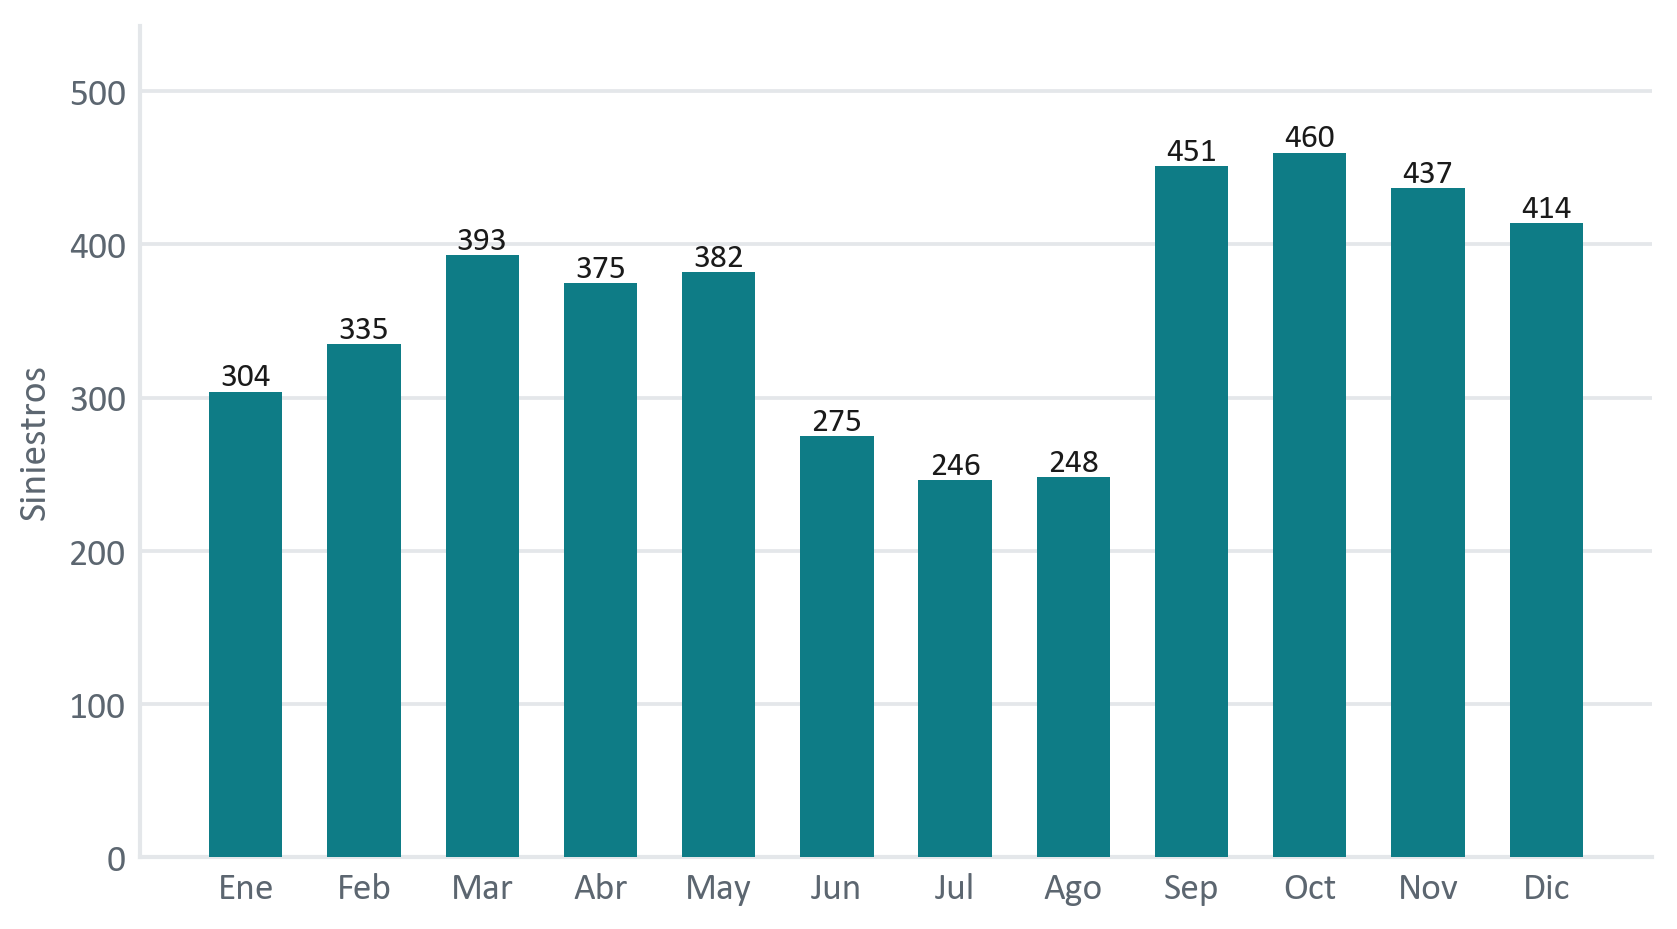
\includegraphics[width=0.92\linewidth]{imagenes/image2.png}
\caption{Distribución de siniestros viales por mes}
\label{fig:distribucion-de-siniestros-viales-por-me}
\notaflot{Frecuencia mensual acumulada de siniestros viales georreferenciados en la ciudad de Córdoba (n = 4320), julio 2022 -- junio 2024. El período de mayor concentración se ubica entre septiembre y diciembre, con un mínimo en julio y agosto. Julio computa únicamente 2023, y agosto 2022 y junio 2024 son meses parciales, por lo que esos tres meses acumulan menos años que el resto. \fuentepropia{} sobre la base de datos de la Unidad Judicial de Accidentología Vial.}
\end{figure}

\begin{figure}[htbp]
\centering
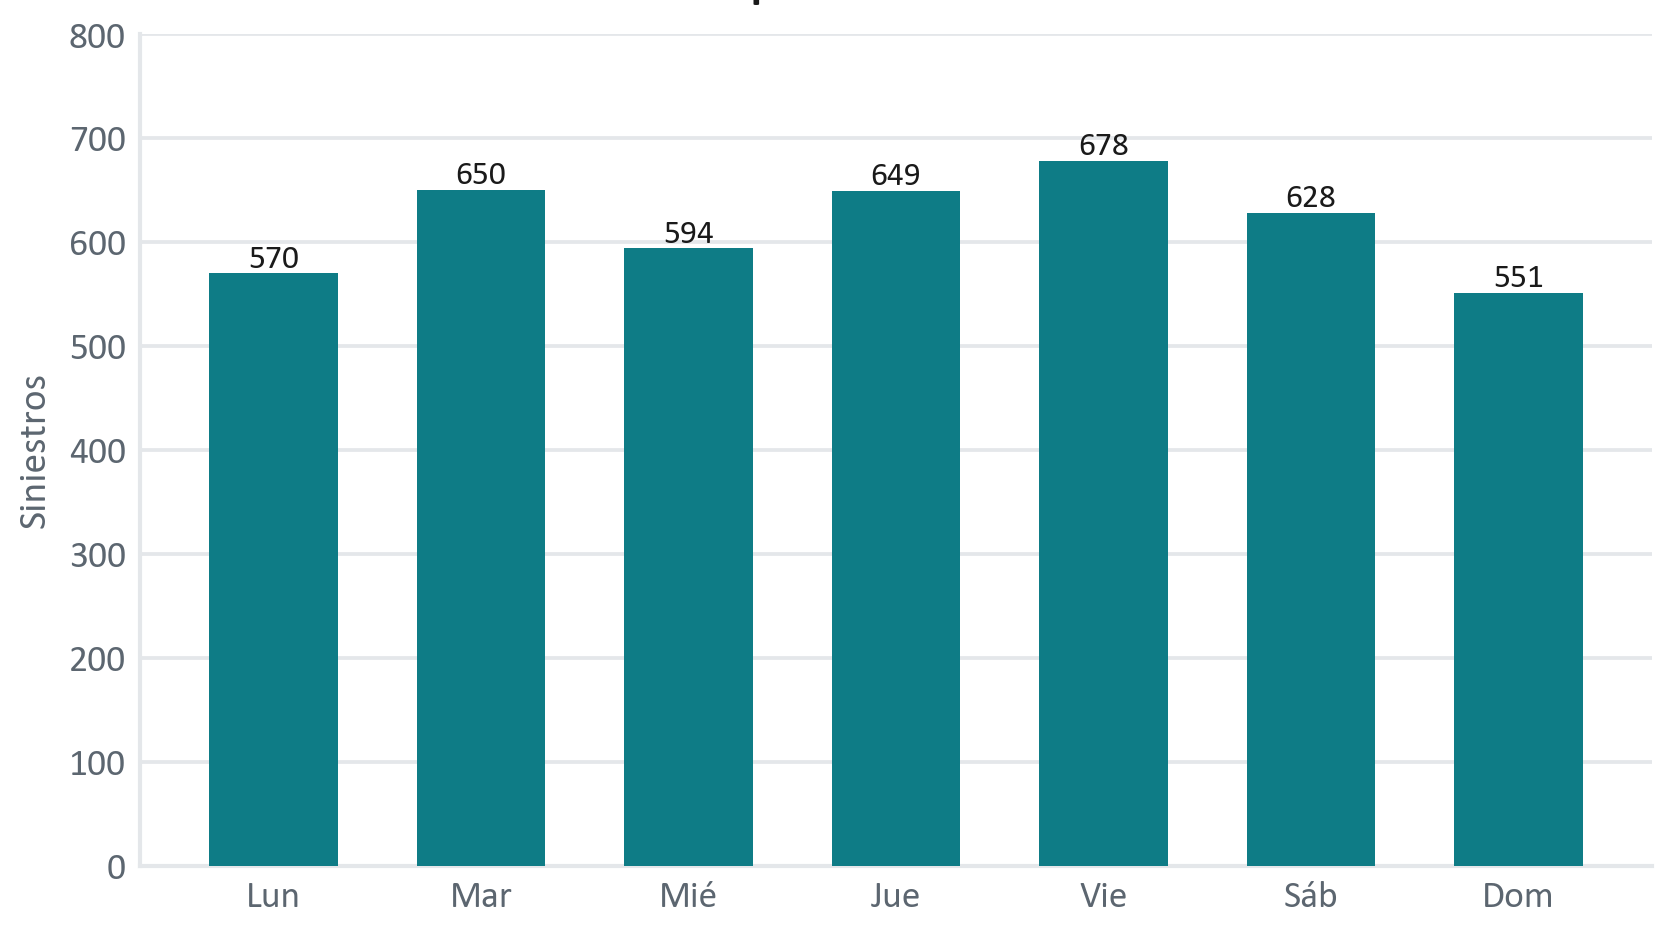
\includegraphics[width=0.92\linewidth]{imagenes/image1.png}
\caption{Distribución de siniestros viales por día de la semana}
\label{fig:distribucion-de-siniestros-viales-por-di}
\notaflot{Frecuencia de siniestros según día de la semana (n = 4320), julio 2022 -- junio 2024. La distribución es relativamente homogénea, con un máximo el viernes (678) y mínimos el domingo (551) y el lunes (570). \fuentepropia{}.}
\end{figure}

\begin{figure}[htbp]
\centering
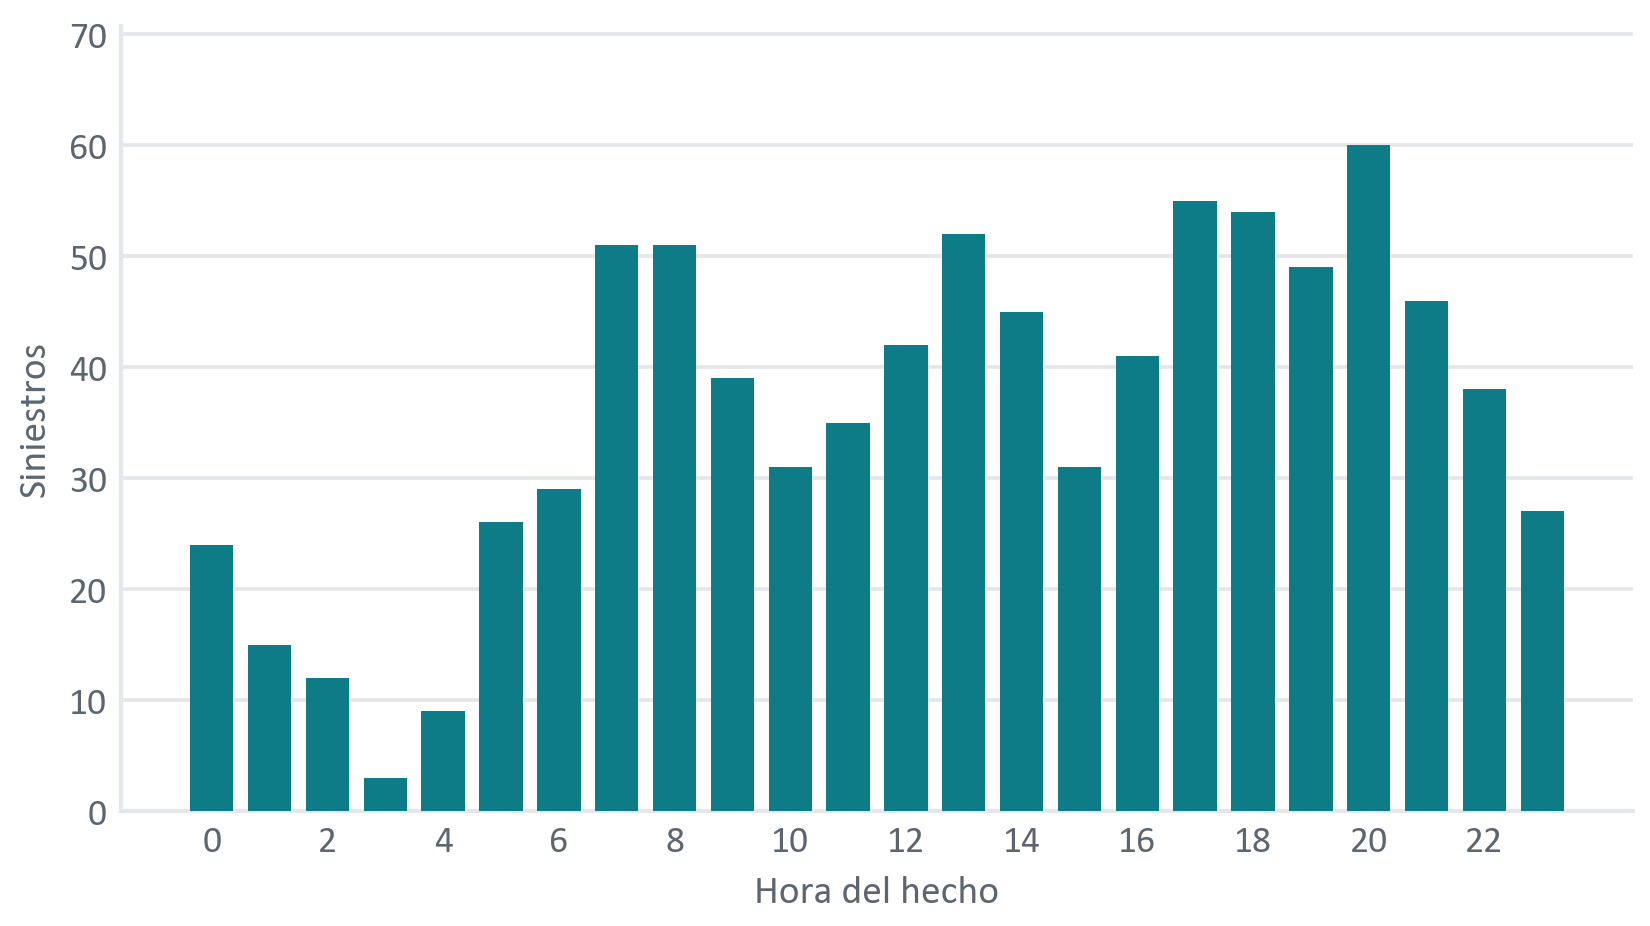
\includegraphics[width=0.92\linewidth]{imagenes/image6.png}
\caption{Siniestros viales por hora del día, año 2022}
\label{fig:siniestros-viales-por-hora-del-dia-ano-2}
\notaflot{Distribución horaria de los siniestros ocurridos durante 2022 (n = 865 registros con hora consignada; 23 casos sin dato, excluidos). Se identifican dos concentraciones asociadas a los desplazamientos cotidianos: una matutina (7 a 9 h) y otra vespertina, más prolongada e intensa (17 a 21 h), con el máximo absoluto a las 20 h. \fuentepropia{}.}
\end{figure}

\begin{figure}[htbp]
\centering
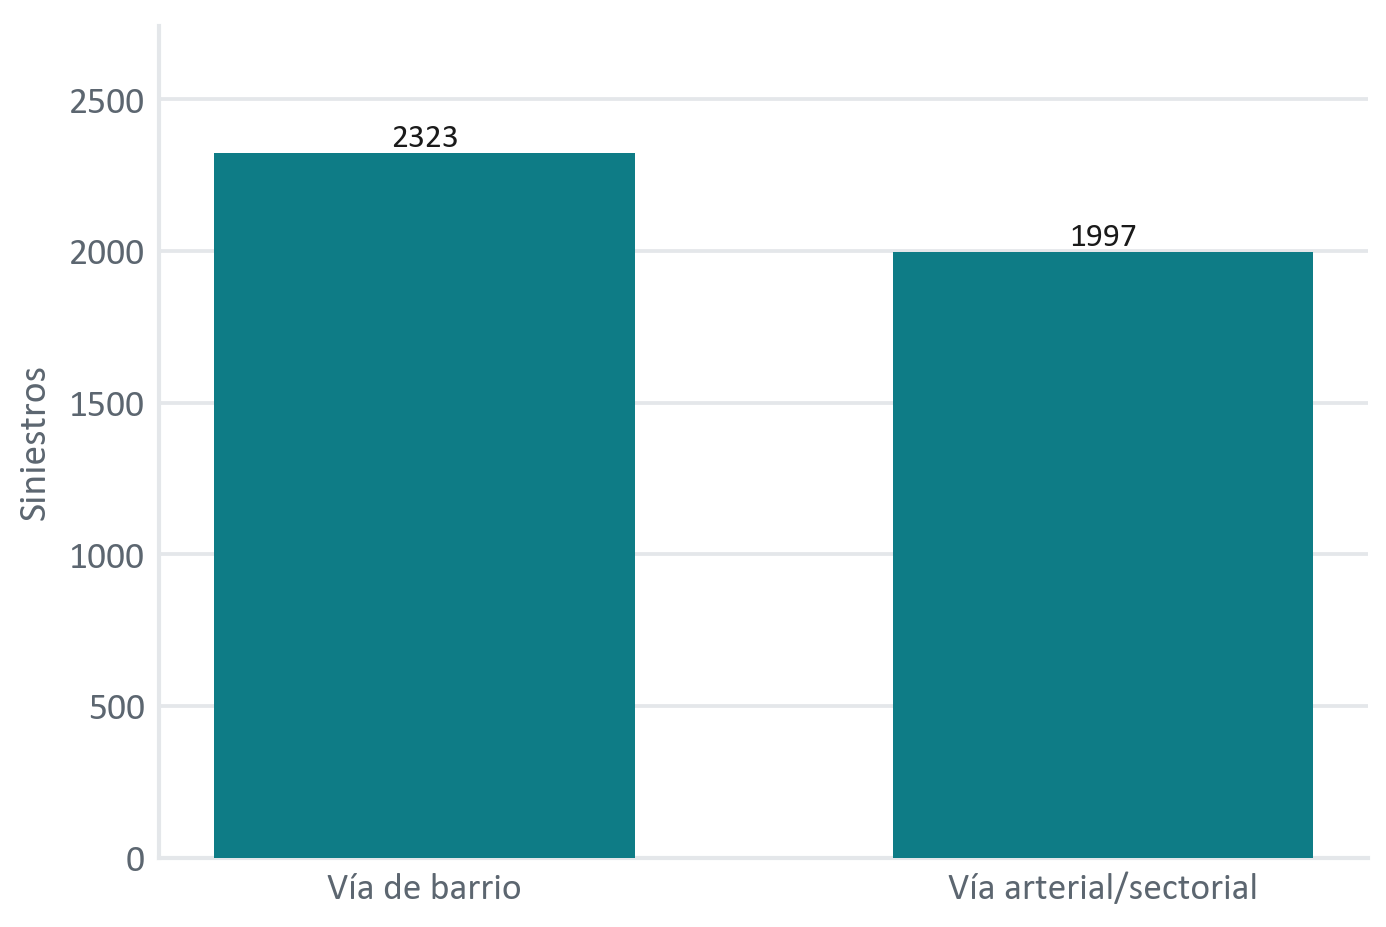
\includegraphics[width=0.78\linewidth]{imagenes/image3.png}
\caption{Distribución de siniestros viales por tipo de calle}
\label{fig:distribucion-de-siniestros-viales-por-ti}
\notaflot{Clasificación de los siniestros según jerarquía de la vía (n = 4320), julio 2022 -- junio 2024. Las vías de barrio concentran 2323 casos y las arteriales o sectoriales 1997, lo que muestra que el fenómeno no se restringe a los corredores principales. \fuentepropia{}.}
\end{figure}

\begin{figure}[htbp]
\centering
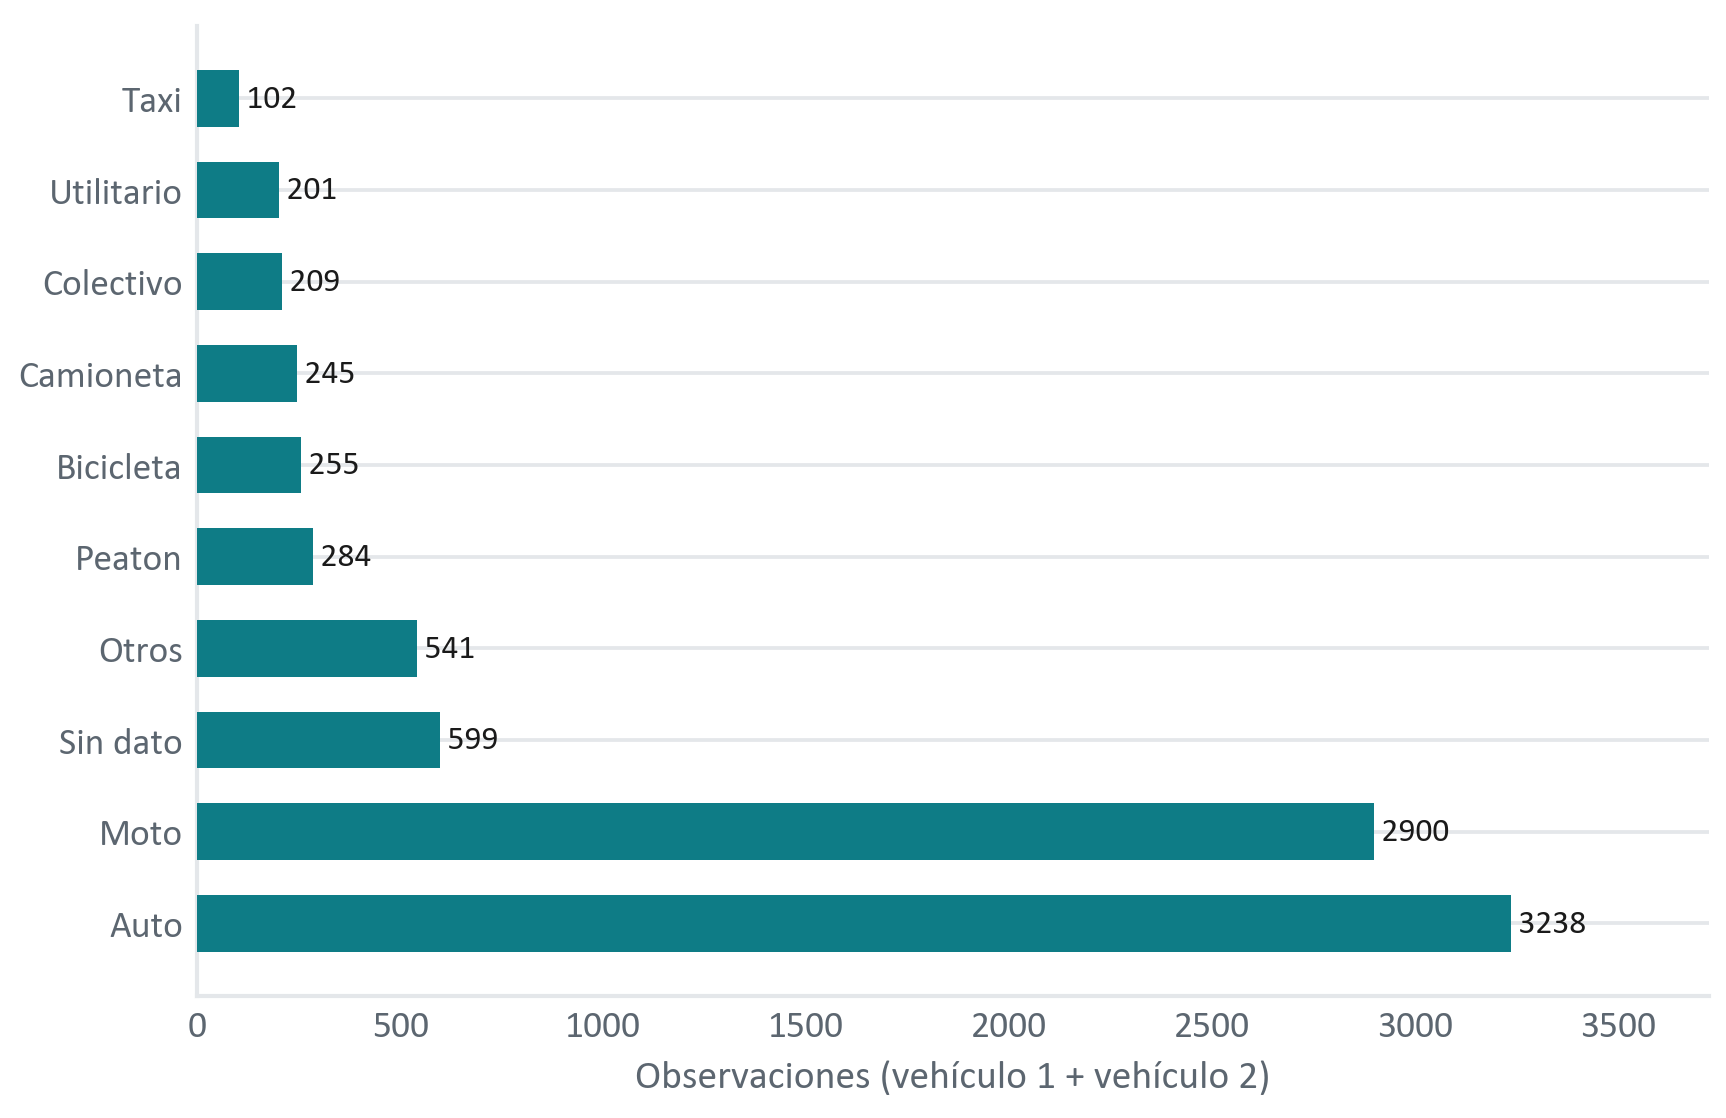
\includegraphics[width=0.81\linewidth]{imagenes/image16.png}
\caption{Distribución del tipo de vehículo o forma de desplazamiento}
\label{fig:distribucion-del-tipo-de-vehiculo-o-form}
\notaflot{Participaciones registradas en los 4320 siniestros (n = 8574 observaciones, correspondientes a vehículo 1 y vehículo 2). La unidad de conteo es la participación y no el siniestro, por lo que las categorías no son excluyentes entre sí. Autos (3238) y motos (2900) concentran la mayor parte de las observaciones. \fuentepropia{}.}
\end{figure}

\begin{figure}[htbp]
\centering
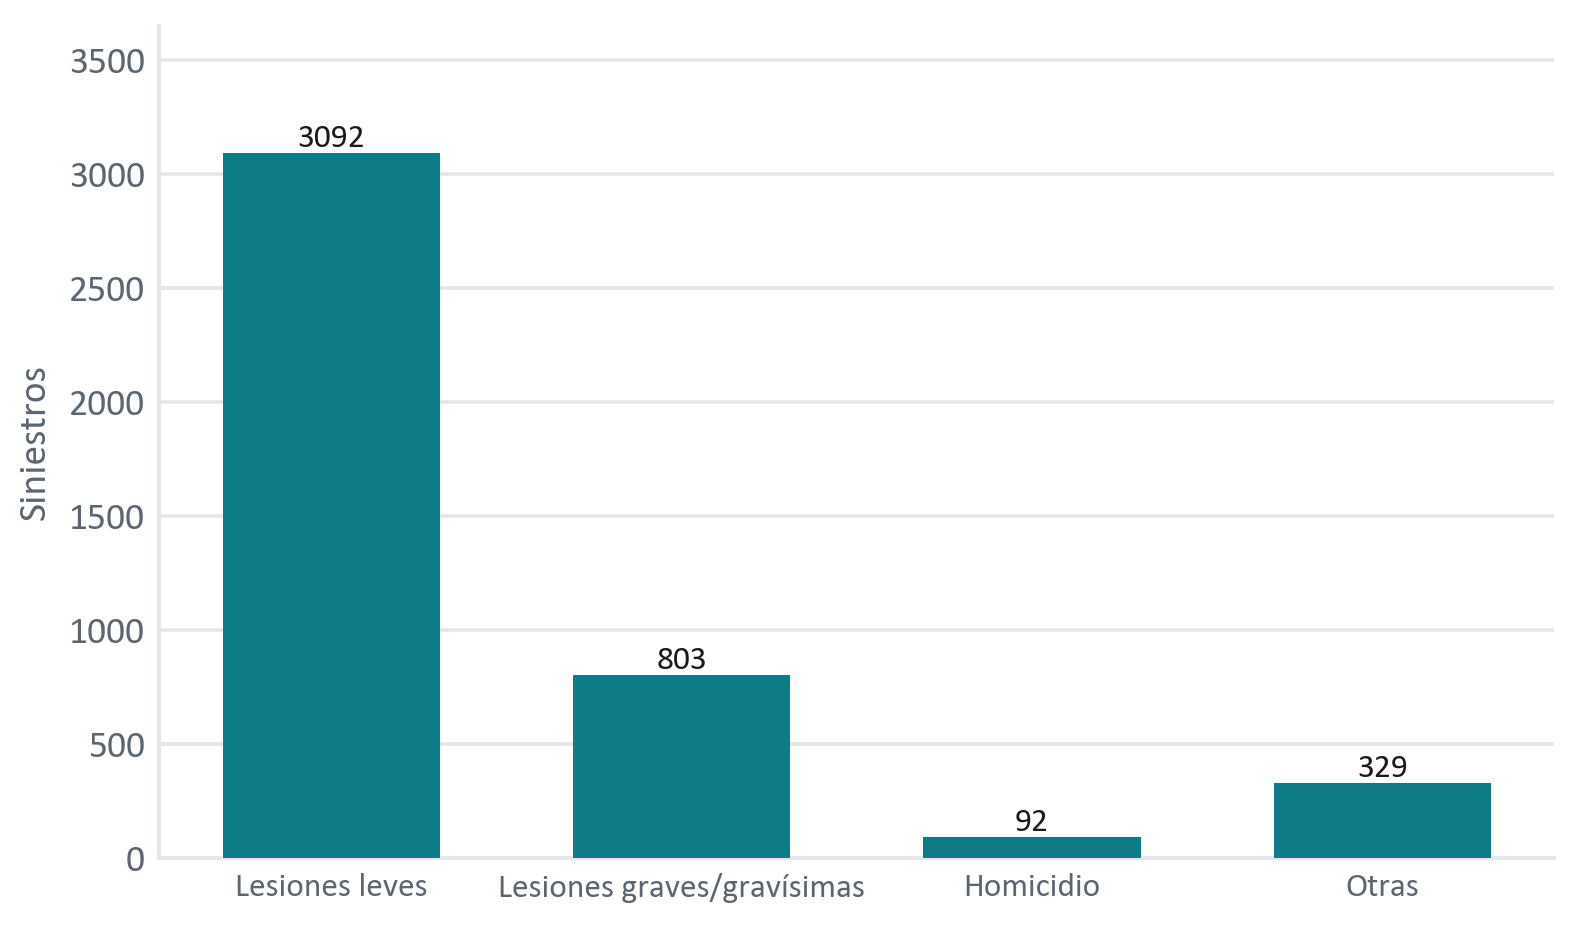
\includegraphics[width=0.89\linewidth]{imagenes/image5.png}
\caption{Distribución de siniestros viales según causa}
\label{fig:distribucion-de-siniestros-viales-segun-}
\notaflot{Clasificación de los siniestros según la carátula asignada en la causa judicial (n = 4316 casos clasificados; 4 sin clasificar, excluidos). Predominan las lesiones leves (3092), seguidas por lesiones graves o gravísimas (803), otras carátulas (329) y homicidio culposo (92). \fuentepropia{}.}
\end{figure}

\begin{figure}[htbp]
\centering
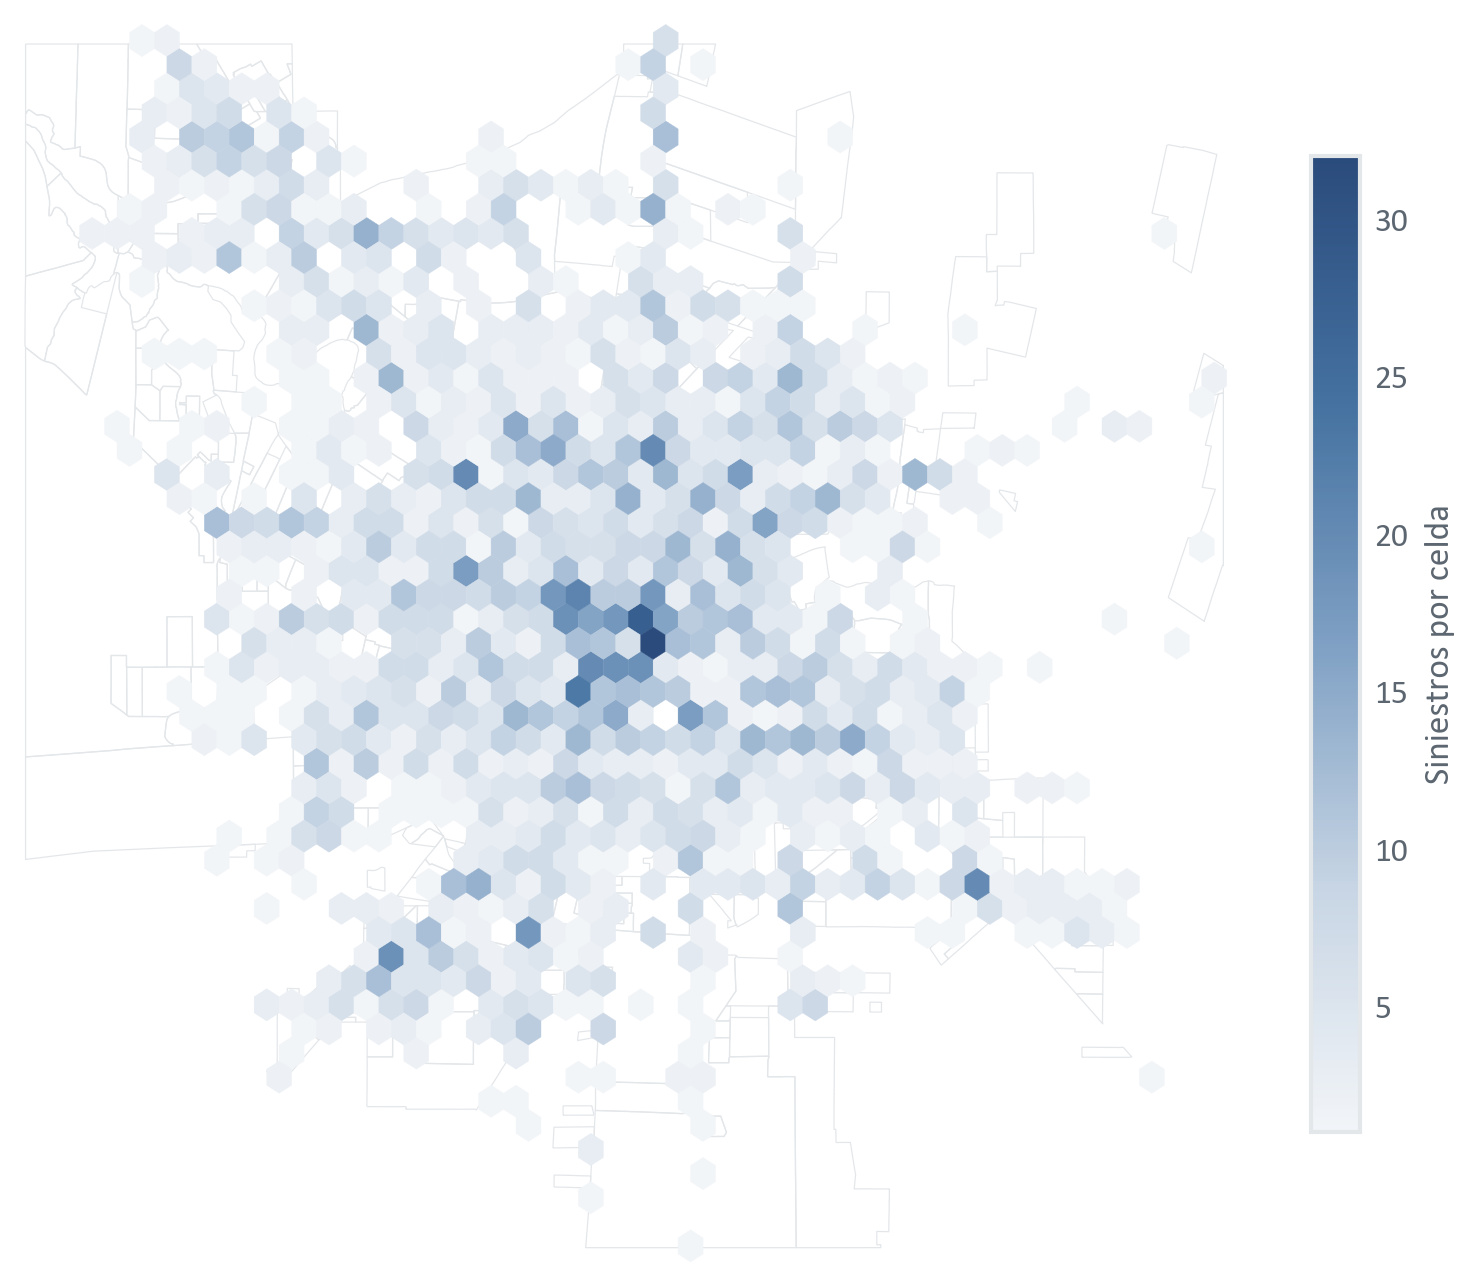
\includegraphics[width=0.92\linewidth]{imagenes/image8.png}
\caption{Mapa de calor de siniestros viales en la ciudad de Córdoba}
\label{fig:mapa-de-calor-de-siniestros-viales-en-la}
\notaflot{Densidad espacial de siniestros georreferenciados (n = 4320), julio 2022 -- junio 2024. La agregación se realiza por celda hexagonal de superficie constante y no por barrio; la silueta de los barrios se incluye solo como referencia visual. Se observa una concentración marcada en el área central y una difusión radial que sigue los principales corredores de acceso. \fuentepropia{}.}
\end{figure}

\section{Antecedentes Relevantes}\label{antecedentes-relevantes}

Una de las tareas que se realizó inicialmente fue la investigación y la búsqueda de antecedentes relevantes, es decir trabajos o publicaciones que fueran sobre el mismo tema o que traten aspectos del enfoque, los datos y las técnicas de aprendizaje automático que sean transferibles o aplicables al producto que se está desarrollando. En este sentido se analizaron principalmente 4 grupos de antecedentes, trabajos sobre accidentología vial de índole analítica o basados en el uso de datos, \eng{forecasting} para problemas similares como incidentes con ambulancias o incendios, sistemas de alerta temprana, ciudades inteligentes, entre otros.

Independientemente del campo de aplicación en el cual se aplicaban los modelos revisados se observaron 3 tipos de enfoques posibles que describen a grandes rasgos las capacidades y requerimientos que se necesitan para un problema con accidentes viales. El primero consiste en trabajar con GNNs, un tipo de arquitectura de redes neuronales basadas en grafos que aprenden patrones de una gran cantidad de datos y que, al procesarlas en sus nodos, permiten generalizar el comportamiento de un sistema. El segundo se basa en el uso de datos georreferenciados. Independientemente del modelo específico utilizado, permite no solo predecir cuándo existe un mayor riesgo de accidentes, sino también dónde es más probable que ocurran. El último consiste en construir una tabla a partir de los registros de accidentes, donde una vez tratada para adaptar el set de datos para que represente una serie temporal se aplican modelos basados en árboles para aprender en qué contexto se incrementa el riesgo de accidentes.

Respecto de los modelos basados en grafos, fueron descartados rápidamente por varios motivos. Si bien se consiguen muy buenos resultados, todos los casos revisados tenían varios órdenes de magnitud adicionales en cantidad de datos, los cuales no eran solamente de accidentes sino que incluyen gran cantidad de variables externas como datos demográficos, información georreferenciada, datos de seguros, criminología, etc. Otra de las motivaciones para desistir por lo menos al inicio en desarrollar un modelo de esta complejidad era el de comenzar con un modelo más simple y si se conseguía buena capacidad de generalización avanzar en estos tipos de sistemas.

El antecedente más significativo para este proyecto es \textcite{novello2022}, que consiste en resolver el mismo problema utilizando inteligencia artificial sólo que aplicado en Ciudad Autonoma de Buenos Aires. La metodología consiste en usar datos georreferenciados y retardos para intentar predecir las zonas con riesgo más elevado. Este enfoque puede categorizarse como sistemas impulsados por modelos espacio-temporales. Respecto de este antecedente, si bien se decidió reproducirlo, hay que tener en cuenta un componente que es determinante para el resultado del mismo, estamos hablando de la densidad de accidentes en el área de trabajo. Los datos para CABA totalizan \num{33234} registros de 29 características cada uno, distribuidos en 3,5 años y \qty{203}{\kilo\metre\squared}. Teniendo en cuenta la cantidad de registros para la Ciudad de Córdoba y el hecho de que tiene 2,8 veces más superficie (\qty{576}{\kilo\metre\squared}), la cantidad de accidentes por unidad de superficie es mucho menor por lo que el desempeño podría verse comprometido.

La última categoría mencionada es la de modelos tabulares basados en árboles. Generalmente requieren una menor cantidad de datos para alcanzar un buen desempeño que enfoques basados en redes neuronales profundas. Para esta metodología se encontró una cantidad considerable de trabajos, por lo que se deja como antecedente general el trabajo de \textcite{zheng2018} en su apartado sobre series temporales.

\section{Experimentación con Modelos}\label{experimentaciuxf3n-con-modelos}

\subsection{LightGBM para Intervalos de Predicción.}\label{lightgbm-para-intervalos-de-predicciuxf3n.}

El primer modelo que se probara consiste en entrenar un LightGBM con el objetivo de hacer un \eng{forecasting} sobre la cantidad de víctimas, la idea de implementar este modelo es que permite ver una línea temporal con la cantidad histórica de víctimas y a partir del punto actual se muestra una línea con el pronóstico esperado más los cuantiles \qty{10}{\percent} y \qty{90}{\percent} (correspondientes al mínimo y al maximo riesgo respectivamente).

Durante el proceso de entrenamiento se decidió crear nuevas variables y características intermedias para intentar mejorar al máximo el rendimiento del modelo, por mencionar algunos: \var{baseline\_60} como un promedio de los últimos 60 días y \var{promedio\_7dias} para los últimos 7 días. Otro aspecto que se debe destacar es que el modelo va a predecir varios bloques horarios de 6 horas, en concreto 28, es decir que el horizonte de predicción es de 7 días.

\begin{longtable}[]{@{}
>{\raggedright\arraybackslash}p{(\linewidth - 4\tabcolsep) * \real{0.3333}}
  >{\centering\arraybackslash}p{(\linewidth - 4\tabcolsep) * \real{0.3333}}
  >{\raggedright\arraybackslash}p{(\linewidth - 4\tabcolsep) * \real{0.3333}}@{}}
\caption{Métricas de rendimiento del modelo LightGBM híbrido L1}
\label{tab:metricas-de-rendimiento-del-modelo-final}\\
\toprule\noalign{}
\textbf{Métrica de Error} & \textbf{Valor} & \textbf{Interpretación} \\
\midrule\noalign{}
\endfirsthead
\toprule\noalign{}
\textbf{Métrica de Error} & \textbf{Valor} & \textbf{Interpretación} \\
\midrule\noalign{}
\endhead
\bottomrule\noalign{}
\endlastfoot
MAE (Mean Absolute Error) & 0,9741 & Medida de ajuste para datos de conteo (valores menores indican mejor ajuste). \\
MASE (Mean Absolute Scaled Error) & 0,1931 & Error Escala Estándar \\
& & \\
\end{longtable}

\notaflot{Métricas calculadas sobre el conjunto de test.}

\begin{figure}[htbp]
\centering
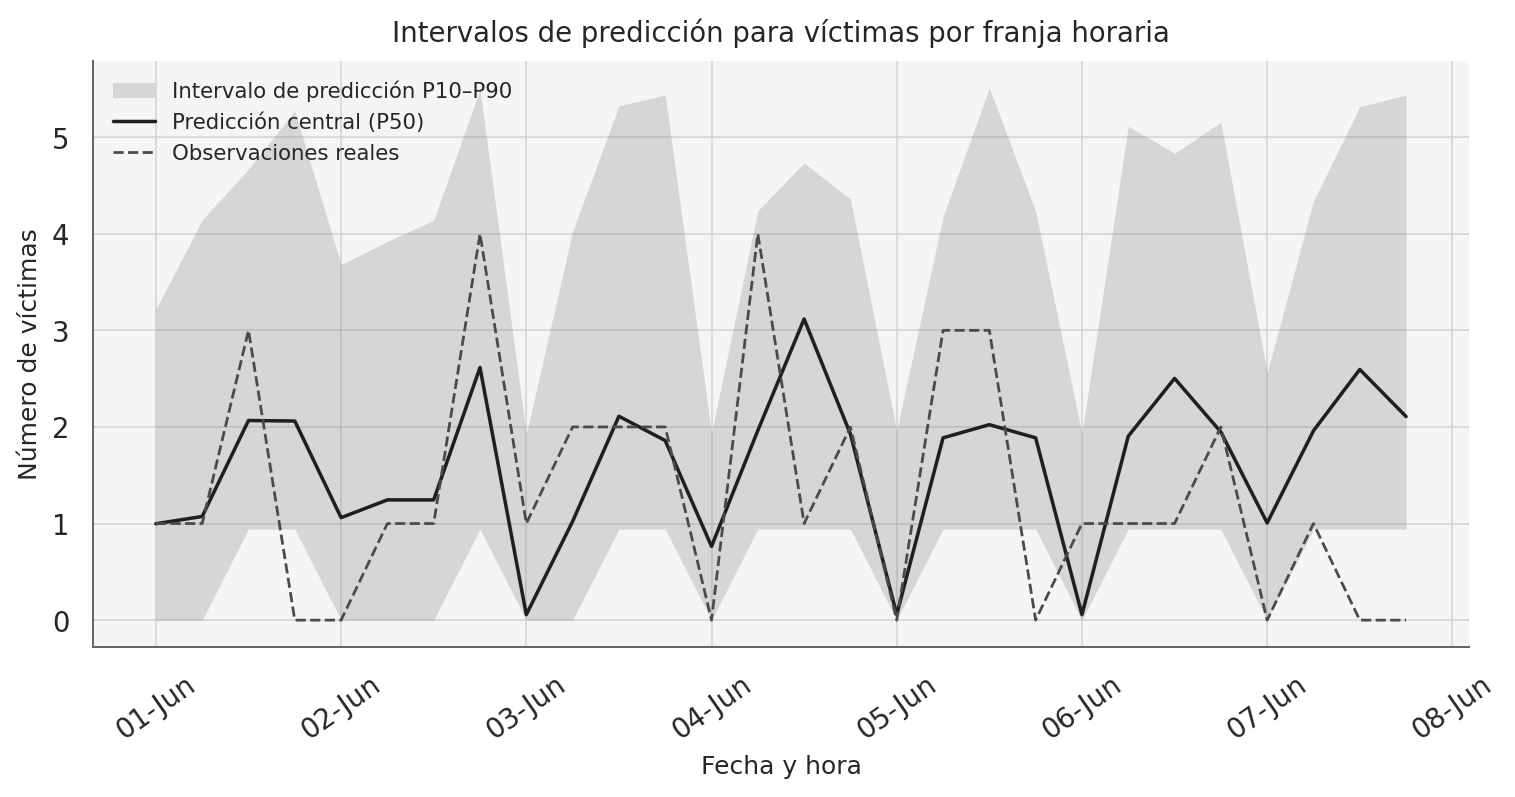
\includegraphics[width=\linewidth]{imagenes/image20.png}
\caption{Pronóstico con LightGBM: predicción central e intervalos P10--P90}
\label{fig:forecasting-lightgbm}
\notaflot{\fuentepropia{}.}
\end{figure}

En la \cref{fig:forecasting-lightgbm} se puede observar que si bien el modelo no se ajusta perfectamente a la realidad, logra identificar cuándo ocurrirán incrementos o descensos en la cantidad de víctimas en toda la ciudad. Este hallazgo sugiere que los datos le permiten a LightGBM aprender patrones de las tendencias de los mismos, y que enriquecerlos con más contexto puede mejorar el ajuste del \eng{forecasting}.

\subsection{Clasificador con Perceptrón Multicapa}\label{clasificador-con-perceptruxf3n-multicapa}

Se quiere probar si proponer una clasificación para los escenarios posibles le facilita a una red neuronal con un perceptrón multicapas alcanzar un buen desempeño. Para ello se generan 3 categorías diferentes a partir de las necesidades que tiene el MPF, las mismas son: Bajo para 2 víctimas o menos, Medio para hasta 4 víctimas y Alto a partir de 5 víctimas en un mismo bloque horario. Los resultados de este experimento se presentan en la \cref{tab:metricas-de-desempeno-multilayer-percept}:

\begin{longtable}[]{@{}
lcccc@{}}
\caption{Métricas de desempeño del clasificador de perceptrón multicapa}
\label{tab:metricas-de-desempeno-multilayer-percept}\\
\toprule\noalign{}
\endfirsthead
\toprule\noalign{}
\endhead
\bottomrule\noalign{}
\endlastfoot
& \textbf{Precisión} & \textbf{Recall} & \textbf{F1-Score} & \textbf{Support} \\
Alto & 0,0909 & 0,0125 & 0,0220 & 80 \\
Bajo & 0,5598 & 0,9035 & 0,6913 & 311 \\
Medio & 0,3469 & 0,0994 & 0,1545 & 171 \\
Accuracy & & & 0,5320 & 562 \\
Macro Avg & 0,3325 & 0,3385 & 0,2893 & 562 \\
Weighted Avg & 0,4283 & 0,5320 & 0,4327 & 562 \\
\end{longtable}

\notaflot{\fuentepropia{}.}

Con solo observar estas métricas podemos ver que el F1 ponderado de 0,4327 es bajo, indica que el desempeño general no es bueno, especialmente cuando se consideran las clases menos frecuentes. El Accuracy (Exactitud) de 0,5320 tampoco es una señal fuerte de buen rendimiento, porque el modelo puede ganar simplemente prediciendo mayoritariamente la clase ``bajo'' (Recall 0,9035). En conclusión se puede decir que segmentar el problema en 3 clases no es suficiente para generar un sistema de alerta temprana de utilidad, al menos en las condiciones actuales.

\subsection{XGBoost Regresor más Capa de Decisión Z-Score}\label{xgboost-regresor-muxe1s-capa-de-decisiuxf3n-z-score}

El problema recientemente mencionado obliga a replantear el enfoque con el cual va a trabajar el próximo modelo. Si generar tres categorías no es suficiente para alcanzar un buen rendimiento entonces se podría proponer un modelo que intente una regresión, es decir que prediga la cantidad exacta de víctimas que habrá y luego aplicar una capa de decisión posterior, la cual le indicará al usuario cual es el riesgo para ese contexto particular.

Para probar que tan bien puede funcionar esta propuesta se propone un XGBoost con 2227 datos para el conjunto de entrenamiento y 557 para el conjunto de prueba. La capa de decisión se ubica a la salida de dicho modelo, comparando la cantidad de víctimas predichas con un promedio histórico para ese contexto según el día y la franja horaria, es decir, si la predicción es de 5 víctimas para un viernes al mediodía entonces compara este valor con el promedio histórico de victimas para todos los viernes al mediodía del pasado. Luego mediante Z-Score ve que tan desviada está la predicción del promedio del pasado, según esta brecha realiza la categorización correspondiente en Bajo, Medio, Alto. Una ventaja que es destacable de este sistema es que permite que en el futuro se pueda calibrar la sensibilidad del modelo al variar los umbrales de Z. Los resultados se presentan en la \cref{tab:metricas-error-xgb-zscore}:

\begin{longtable}[]{@{}
>{\raggedright\arraybackslash}p{(\linewidth - 4\tabcolsep) * \real{0.3333}}
  >{\centering\arraybackslash}p{(\linewidth - 4\tabcolsep) * \real{0.3333}}
  >{\raggedright\arraybackslash}p{(\linewidth - 4\tabcolsep) * \real{0.3333}}@{}}
\caption{Métricas de error del XGBoost regresor con capa Z-Score}
\label{tab:metricas-error-xgb-zscore}\\
\toprule\noalign{}
\textbf{Métrica de Error} & \textbf{Valor} & \textbf{Interpretación} \\
\midrule\noalign{}
\endfirsthead
\toprule\noalign{}
\textbf{Métrica de Error} & \textbf{Valor} & \textbf{Interpretación} \\
\midrule\noalign{}
\endhead
\bottomrule\noalign{}
\endlastfoot
Poisson Deviance & 1,6627 & Medida de ajuste para datos de conteo (valores menores indican mejor ajuste). \\
MSE (Error Cuadrático Medio) & 1,2926 & Promedio de los errores cuadráticos entre el valor real y predicho. \\
RMSE (Raíz del Error Cuadrático Medio) & 1,137 & Desviación promedio del modelo. \\
\end{longtable}

\notaflot{Métricas calculadas sobre el conjunto de test independientemente del umbral de clasificación.}

\begin{figure}[htbp]
\centering
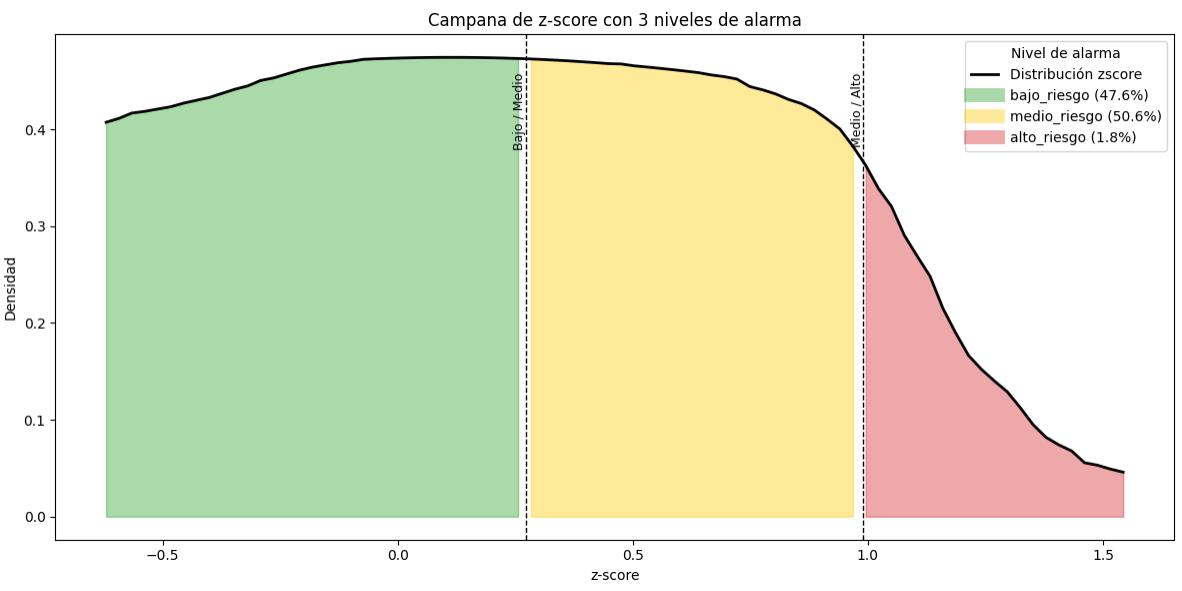
\includegraphics[width=\linewidth]{imagenes/image19.png}
\caption{Capa de decisión Z-Score y su distribución}
\label{fig:capa-de-decision-z-score-y-su-distribuci}
\notaflot{\fuentepropia{}.}
\end{figure}

Si bien las métricas no se pueden tomar como 100 por ciento satisfactorias, este modelo puede ser de mayor utilidad en comparación a los que se mencionaron hasta ahora, esto es debido a que si se exploran algunas nuevas variables que puedan contribuir a la mejoras de las métricas o si con el transcurso del tiempo estas mejoran debido al aumento en la cantidad de datos para entrenar, y se considera también el hecho de que tiene umbrales regulables que permiten ajustar las alertas a necesidad y criterio del usuario final, entonces puede considerarse seriamente para implementarlo en el MVP.

\subsection{Perceptrón Multicapa Binario con Capa de Decisión.}\label{perceptruxf3n-multicapa-binario-con-capa-de-decisiuxf3n.}

Considerando la metodología anterior, referida al uso de una capa de decisión posterior a la predicción del modelo, surge la pregunta entonces de qué pasaría con el desempeño del sistema en su conjunto si reemplazamos el XGBoost por un MLP. Se realizará entonces un experimento para comprobar cual de los dos modelos obtiene el mejor rendimiento para emitir las alertas.

En este caso es necesario recordar que las características del dataset son las mismas que en el XGBoost, esto es porque el objetivo es aislar el efecto del modelo para conocer exactamente cuánta es la contribución del MLP a la clasificación final. No obstante varía en cuanto a la naturaleza del atributo objetivo, el mismo es binario, es decir que el modelo tiene por salida una variable continua entre 0 y 1. Luego se procesan los quantiles para clasificar.

\begin{longtable}[]{@{}
>{\raggedright\arraybackslash}p{(\linewidth - 2\tabcolsep) * \real{0.3340}}
  >{\centering\arraybackslash}p{(\linewidth - 2\tabcolsep) * \real{0.3340}}@{}}
\caption{Métricas del perceptrón multicapa binario con capa de decisión}
\label{tab:resumen-de-metricas-del-modelo}\\
\toprule\noalign{}
\textbf{Métrica} & \textbf{Valor} \\
\midrule\noalign{}
\endfirsthead
\toprule\noalign{}
\textbf{Métrica} & \textbf{Valor} \\
\midrule\noalign{}
\endhead
\bottomrule\noalign{}
\endlastfoot
AUC-ROC & 0,6289 \\
Brier Score & 0,2053 \\
\end{longtable}

\notaflot{\fuentepropia{}.}

\subsection{XGBoost, Modelo Georreferenciado}\label{xgboost-modelo-georreferenciado}

Para desarrollar el modelo de forma tal que pase de ser solo temporal a espacio-temporal hay que realizar algunas consideraciones y tomar algunas decisiones importantes para adaptar esta solución a la ciudad de Córdoba.

La primera decisión que se tomó consistió en determinar de qué tamaño iban a ser las cuadrículas en la ciudad, inicialmente se propuso \qty{500}{\metre} por \qty{500}{\metre} en función del trabajo que se revisó \autocite{novello2022}, luego de un análisis estadístico se determinó que convenía hacer una cuadricula de \qty{1000}{\metre} por \qty{1000}{\metre} y si el modelo generaliza bien se podía reducir y evaluar los resultados.

Se tiene entonces la ciudad de Córdoba dividida en una cuadrícula como la mencionada, cada día tiene 4 bloques horarios de 6 horas, entonces cada combinación de área más rango horario es una fila del set de datos. Teniendo en cuenta que la ciudad tiene \qty{576}{\kilo\metre\squared} los registros totalizan \num{1472000} filas, de las cuales el \qty{0.28}{\percent} tienen accidentes. Este último número es la dificultad central del problema, un modelo que siempre predijera que no va a pasar nada acertaría el \qty{99.7}{\percent} de las veces. La \cref{fig:esquema-del-modelo-georreferenciado-impu} representa el proceso de entrenamiento.

\begin{figure}[htbp]
\centering
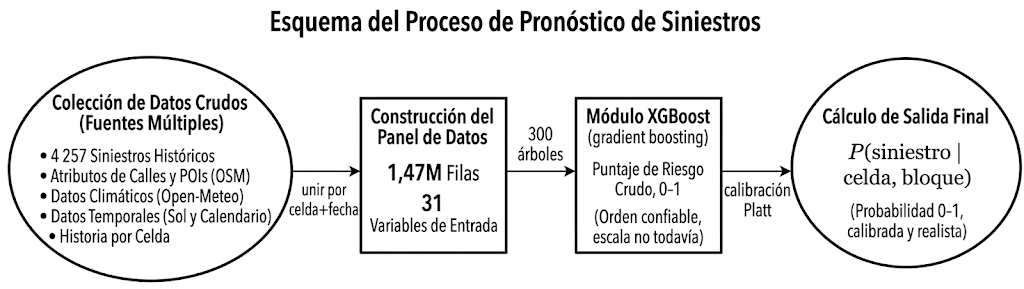
\includegraphics[width=\linewidth]{imagenes/image18.png}
\caption{Esquema del modelo georreferenciado impulsado por XGBoost}
\label{fig:esquema-del-modelo-georreferenciado-impu}
\notaflot{\fuentepropia{}.}
\end{figure}

Si bien este modelo obtuvo resultados modestos, promedio PR-AUC 0,0097 vs 0,0085 del promedio histórico; ROC-AUC 0,809 vs 0,778, permitió obtener información valiosa acerca del problema que se tendrá en cuenta cuando se desarrolle el modelo final. A forma de resumen podemos decir que la forma correcta de testear el modelo es usando Walk Forward, se debe evitar usar calibración isotónica cuando se tienen pocos casos positivos reemplazandola por Platt Scaling, y por último, se puede afirmar que el enfoque de trabajo georreferenciado funciona (el modelo ganó 5 veces ) y que si en el futuro se continúan recolectando datos tiene un gran potencial para crecer en cuanto a rendimiento.

En la sección siguiente se toman estas métricas como punto de partida, y se hace un resumen para sumarizar los hallazgos e indicios que se obtuvieron del proceso experimental.

\section{AutoGluon-TimeSeries}\label{autogluon-timeseries}

En la etapa final de exploración de modelos se desarrolló un proyecto en el Centro de Cómputos de Alto Desempeño de la Universidad Nacional de Córdoba (CCAD-UNC), el mismo consta de aplicar a los datos de este problema el pipeline de auto ML de AutoGluon-TimeSeries. Como se explicó en secciones anteriores este paso permite entrenar varios modelos simultáneamente para obtener una combinación óptima que maximice la performance.

\subsection{Configuración del Modelo AutoGluon y entrenamiento en CCAD}\label{configuraciuxf3n-del-modelo-auto-gluon-y-entrenamiento-en-ccad}

Se configuró el predictor de series temporales de AutoGluon (TimeSeries Predictor) para optimizar la métrica MASE sobre la variable objetivo en escala logarítmica (\var{victimas\_log}), ajustando los datos a una frecuencia de 6 horas con estacionalidad diaria ($m = 4$) y un horizonte de predicción de 14 días (56 pasos). Se definieron como covariables conocidas variables de calendario y contexto (\var{dia\_semana\_cat}, \var{es\_fin\_de\_semana}, mes y \var{tipomesESCOLAR}). El entrenamiento se ejecutó bajo el perfil \enquote{\var{high\_quality}} con un tiempo total de 12 horas, utilizando una estrategia de validación cruzada temporal (\eng{walk-forward}) de 4 ventanas consecutivas para garantizar una evaluación robusta sobre el histórico de datos.

\begin{longtable}[]{@{}
lcccc@{}}
\caption{Resultado del proceso de ensamble ponderado de AutoGluon}
\label{tab:resultado-del-proceso-de-ensamble-ponder}\\
\toprule\noalign{}
\textbf{Modelo} & \textbf{Score Test} & \textbf{Score Val} & \textbf{T Pred} & \textbf{T Ajuste} \\
\midrule\noalign{}
\endfirsthead
\toprule\noalign{}
\textbf{Modelo} & \textbf{Score Test} & \textbf{Score Val} & \textbf{T Pred} & \textbf{T Ajuste} \\
\midrule\noalign{}
\endhead
\bottomrule\noalign{}
\endlastfoot
Direct Tabular & -0,6983 & -0,8229 & 0,11 & 4,32 \\
DeepAR & -0,7011 & -0,8143 & 9,30 & 117,78 \\
Weighted Ensemble & -0,7116 & -0,7823 & 13,17 & 1,66 \\
Auto ETS & -0,7252 & -0,8077 & 4,25 & 72,69 \\
TFT & -0,7314 & -0,7911 & 0,40 & 416,63 \\
\end{longtable}

\notaflot{Los valores de Score corresponden a la métrica MASE invertida (multiplicada por -1), donde valores más cercanos a 0 indican mejor rendimiento. Los tiempos de predicción (T. Pred.) y ajuste (T. Ajuste) están expresados en segundos.}

Como se puede observar en estos resultados, el mejor desempeño lo tiene Direct Tabular, que en AutoGluon corresponde a modelos XGBoost o LightGBM configurados con ventanas deslizantes, lo que confirma las hipótesis de trabajos con las que se desarrollaron los modelos anteriores y se alinea con los antecedentes citados durante este proyecto.

\subsection{Resumen de Hallazgos en Experimentos}\label{resumen-de-hallazgos-en-experimentos}

En esta sección se analizarán los hallazgos de la etapa de experimentación teniendo en cuenta no sólo las métricas de los modelos, sino también expandiendo el análisis para contemplar otros criterios que no pueden obviarse si se quiere obtener una solución que se ajuste a las necesidades del usuario y su contexto.

El primer aspecto a tratar es cómo se va a predecir la variable objetivo, habiéndo se trabajado en dos posibilidades, las regresiones para valores continuos en la cantidad de víctimas y las clasificaciones tanto binarias como en diferentes categorías. Los hallazgos sugieren que a todos los modelos entrenados les cuesta identificar momentos de bajo riesgo independientemente de cómo se le pida la salida a los mismos, tomando el caso por ejemplo del MLP en clasificación binaria con una curva AUC-ROC de 0,6289 o el caso de XGBoost con Recall de 0,39 (identificó sólo el \qty{39}{\percent} de los momentos en donde no hubo accidentes viales) en momentos seguros y 0,87 para momentos críticos (este modelo se desarrolla con más profundidad en el siguiente apartado). De los demás experimentos realizados se puede dejar como observación que el LightGBM que se configuró para mostrar la línea de predicción más intervalos P10 y P90 logra identificar mejor los momentos seguros que las otras variantes.

El siguiente hallazgo puede resumirse en que si se compara el desempeño de los modelos clasificadores contra los regresores resulta notablemente mejor hacer un sistema híbrido compuesto por un modelo regresor y una capa de decisión adicional que clasifique el riesgo luego de hacer la predicción. En este sentido se destaca el XGBoost Regresor con capa de decisión Z-Score en comparación por ejemplo con el MLP que clasifica directamente en Alto, Medio y Bajo que solo tiene un desempeño aceptable en una de sus clases.

A lo largo de todo el proceso de experimentación se pudo confirmar mediante la realización de entrenamientos con múltiples modelos y búsqueda por grilla de hiperparámetros que el fenómeno puede explicarse principalmente por el comportamiento histórico de la cantidad de víctimas y algunas variables representativas del dia de la semana y el rango horario que se está observando. Es decir que no se observaron contribuciones significativas a la capacidad predictiva de variables como la temperatura, la presión, el periodo escolar y otras variables. Este aspecto se encuentra mejor explicado en la sección de resultados del modelo de línea de base.

Respecto del modelo de línea de base, se optó por seleccionar XGBoost configurado para regresión de Poisson, el motivo de esto es obtener un modelo que pueda ser usado de base de comparación para medir la evolución de futuros reentrenamientos, mejoras, adaptaciones, y también de cómo evoluciona la capacidad de predicción cuando se incorporen nuevos datos. Si bien este modelo termina por clasificar de forma binaria la ocurrencia de un siniestro, solo lo hace definiendo un umbral fijo predefinido. Esta decisión no se tomó arbitrariamente, es necesario usar de línea de base la capacidad predictiva propia del modelo, aislandolo de los efectos del uso posterior de capas de decisión como las Z-Score.

\section{Pipeline del Modelo de Línea Base (Baseline)}\label{pipeline-del-modelo-de-luxednea-base-baseline}

En esta instancia se explicará cómo se generó el modelo de línea de base para este proyecto, usualmente se trabaja con un modelo que tiene una complejidad relativamente baja respecto de otras técnicas, con el objetivo de experimentar rápidamente y testear diferentes hipótesis que permitan confirmar si los datos tienen la calidad y cantidad suficiente \autocite{zheng2018} como para que un determinado modelo pueda adquirir una capacidad de generalización útil para el fin en cuestión. En este caso se decidió comenzar con un árbol de decisión XGBoost por el hecho de que permite recuperar información acerca de la importancia de cada variable para generar la predicción, esto es un insumo fundamental para realizar uno de los procesos fundamentales del Machine Learning que es denominado ingeniería de características y que es el que permite comprender mejor la naturaleza del fenómeno estudiado.

La estructura definida en el apartado anterior es de gran valor a la hora de comprender el problema que se quiere abordar, es lo suficientemente específica, amplia en el sentido de contener muchas características y adecuado para aplicar modelos de distintos tipos como pueden ser clasificadores para buscar patrones en grupos o modelos de analítica descriptiva más clásicos que permitan obtener información valiosa. Esto es posible porque el dataset contiene mucha información que caracteriza cada hecho en particular, como por ejemplo el tipo de vehículo involucrado, datos sobre las personas involucradas, distancia al semáforo más próximo, datos de referenciación geográfica, entre otros. Sin embargo, la forma en la que esta información está estructurada no es útil para la realización de \eng{forecasting} para un sistema que pretende anticipar en una ventana de tiempo la cantidad de víctimas o lesionados que pudiera haber, esto es por un motivo trivial, cuando trabaja con series temporales se utiliza información disponible en el momento o que se tiene del pasado para poder realizar la predicción, pero en todos los casos tiene que ser información disponible antes del suceso que se quiere pronosticar. El formato en el que se encuentran los datos actuales es denominado Tabla de Hechos, y consiste básicamente en que cada fila es un registro de un hecho puntual en un determinado momento, es decir que de manera general contiene la fecha y hora, y en las columnas consecutivas información relevante del evento.

Uno de los principales aspectos que debió reformularse al inicio del proyecto es el derivado de la propia naturaleza de la tabla de hechos, la cual no registra el tiempo de manera continua, es decir, que los días en los que no hay accidentes no se tiene información, esto es especialmente relevante para diseñar una alerta temprana dado que es de vital importancia saber bajo qué condiciones no ocurren accidentes. Para solucionar este problema se optó por dividir un cada día en bloques de 6 horas, de manera tal que la cantidad de accidentes que corresponden a un mismo bloque horario se suman para representar el riesgo de tal, cuando no existan accidentes el bloque contiene un cero para indicarle al modelo que no pasó nada. Las demás variables son agregadas de igual manera según criterios convenientes de manera tal que representen lo mejor posible a cada bloque, por ejemplo para la temperatura se toma el promedio durante las 6 horas correspondientes. Es importante destacar que la decisión de dividir el día en 4 bloques de 6 horas cada uno no es arbitraria sino que fue tomada en base a experiencias del personal del ministerio público fiscal y consultada con distintos especialistas pertenecientes a LIDeSIA.

\begin{figure}[htbp]
\centering
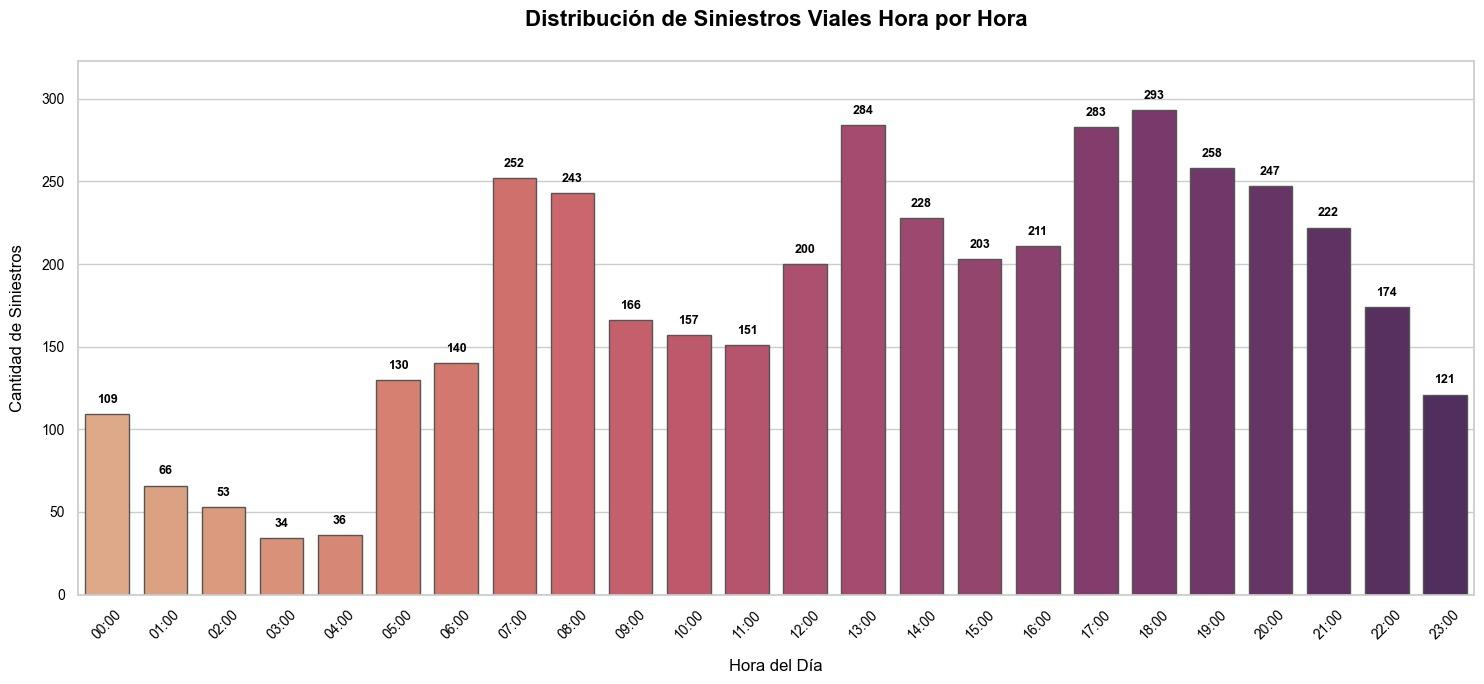
\includegraphics[width=\linewidth]{imagenes/image23.jpg}
\caption{Distribución del total de accidentes por hora del día}
\label{fig:distribucion-del-total-de-accidentes-por}
\notaflot{\fuentepropia{}, a partir de los datos provistos por el Ministerio Público Fiscal.}
\end{figure}

Continuando con las estrategias implementadas para poder aplicar un modelo XGBoost (Extreme Gradient Boosting) se explicará cómo se modificó el set de datos para cambiar la forma en que representa la información. El objetivo final es que cada registro ordenado cronológicamente contenga información dividida en tres partes, datos del pasado, datos del presente, y la cantidad de accidentes que hubo en ese contexto.

Para esto se utilizará un enfoque llamado Formulación Autorregresiva Supervisada que consiste en traer al presente información del pasado por medio de retardos (Lags) y sumarlo a los datos del presente para generar el contexto que explique la cantidad de víctimas que hubo en ese momento. Un ejemplo de esto puede ser la propia cantidad de víctimas de un bloque horario de 6 horas, por ejemplo, para un dia viernes por la tarde reconstruirse información del pasado trayendo al presente el promedio de víctimas de la última semana, las víctimas del viernes anterior, las víctimas de las últimas 12 horas e infinidad de combinaciones posibles que se pueden generar con esta y otras variables como las climáticas por ejemplo. Siguiendo este método, para generar un registro basta con crear un algoritmo que se desplace pasos hacia atrás en el tiempo, agregue la información que se requiere y la inscriba en el registro actual.

Nótese de esta manera que lo que representan los datos cambió totalmente, antes se tenía una serie de registros que ubican cada accidente en particular de manera irregular y con información que caracteriza el hecho en sí, ahora en cambio, se tiene un set de datos que representa el estado de un sistema (Tránsito de la Ciudad de Córdoba) definido por una serie de características las cuales al variar en el tiempo generar incrementos o decrementos del riesgo de accidente vial. Una vez que el modelo sea entrenado, el mismo aprenderá a detectar los patrones que generan una subida en la cantidad de víctimas registradas, así como qué combinación de variables hace que el riesgo del sistema de tránsito permanezca bajo.

\begin{figure}[htbp]
\centering
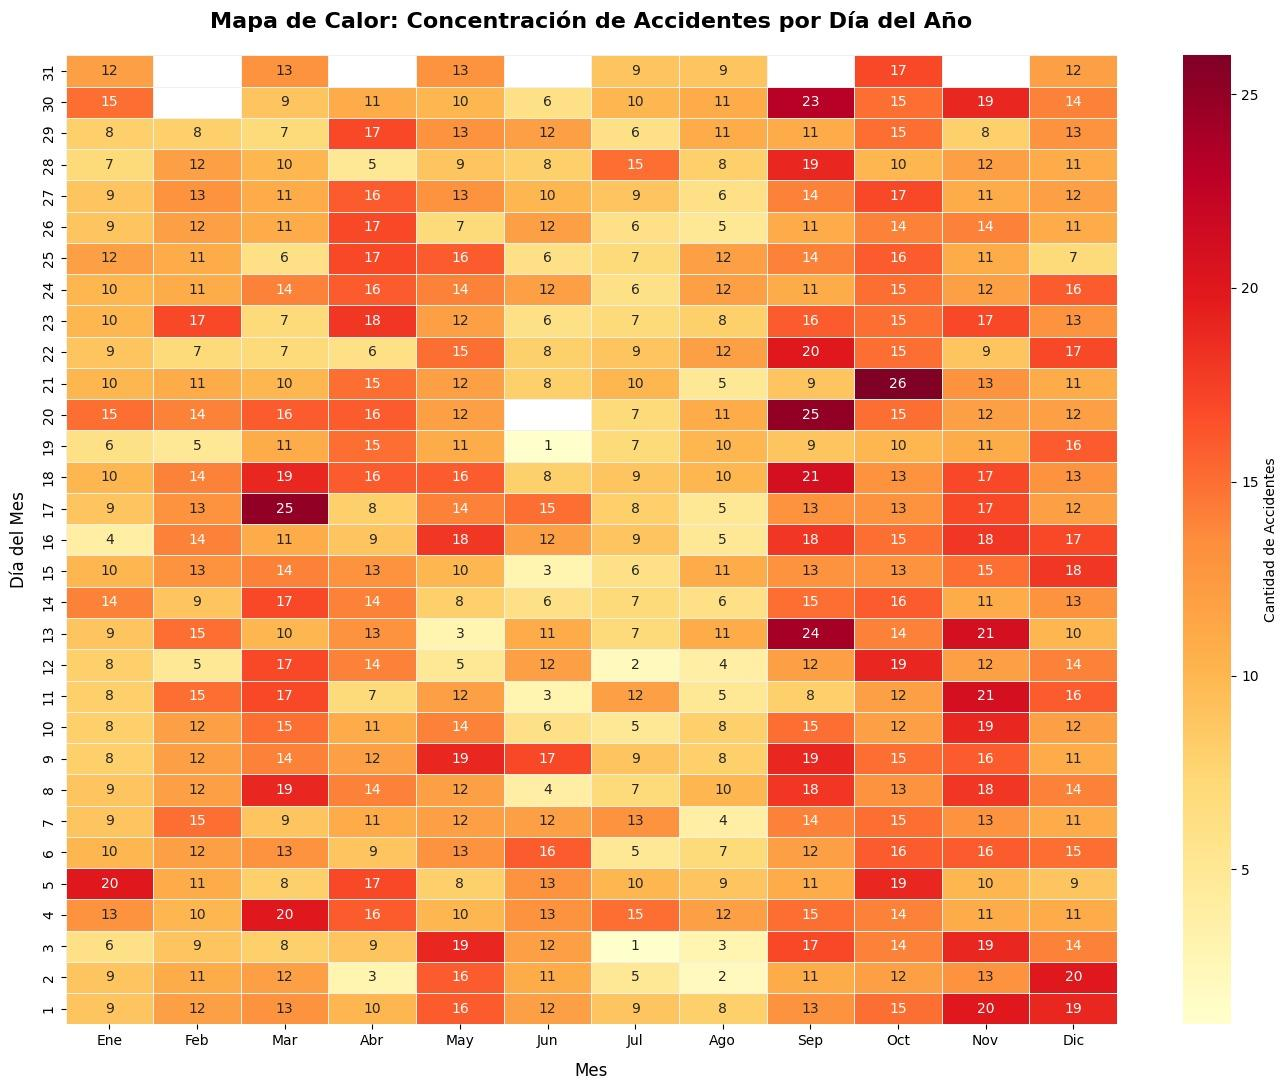
\includegraphics[width=\linewidth]{imagenes/image24.jpg}
\caption{Concentración de accidentes por día del año}
\label{fig:mapa-calor-dia-anio}
\notaflot{\fuentepropia{}.}
\end{figure}

\subsection{Definición de la estructura de Ventanas Deslizantes}\label{definiciuxf3n-de-la-estructura-de-ventanas-deslizantes}

En este punto se comienza definiendo la variable objetivo para el entrenamiento de Machine Learning, la variable objetivo es la que el modelo intenta predecir a partir de las demás características o features que aporta el set de datos. Para este caso se definió una variable denominada en el dataset como \var{TARGET\_CRITICO} la cual es de naturaleza binaria, es decir que toma el valor de 1 cuando existe al menos una víctima de accidente vial y 0 cuando no pasó nada. La relación con el formato de ventana deslizante consiste en que esta variable será la que permite calcular los retardos que se mencionan más adelante.

Por otro lado se tienen las variables relacionadas a la dimensión del tiempo, como por ejemplo el día está codificado con un 1 para el Lunes, 2 para el Martes y así sucesivamente. Análogamente se categorizaron las franjas horarias en este caso 1 significa la franja que va desde las 00:00 horas hasta las 06:00 horas, el 2 es el bloque contiguo, lo mismo ocurre con la variable mes del año en cuestión. En las variables que refieren al tiempo puede ocurrir un problema dependiendo el modelo que se esté utilizando, este radica en el hecho de que el mismo no entiende que el tiempo es cíclico en el sentido que para el algoritmo el lunes está a una distancia de 6 respecto al domingo, cuando en realidad también los separa una distancia de 1. En este caso tenemos la posibilidad de aplicar una transformación seno coseno a cada una de estas variables solucionando el inconveniente anterior. En el caso de árboles de decisión su uso no es del todo recomendable porque puede generar inconvenientes, pero es necesario aclararlo por si en el modelo definitivo se deciden usar modelos complementarios como el Perceptrón Multicapa por ejemplo.

Si se tiene presente la estrategia de las ventanas deslizantes para traer de forma autorregresiva información del pasado al presente para predecir el futuro, es razonable plantearse que no solo una agregación de las últimas víctimas que hubo en horas pasadas puede ser suficiente para poder hacer un \eng{forecasting} con algún grado de precisión, en cambio conviene generar adecuadamente un tipo de variable que indique tendencias o inercia, esto es por que se sospecha que si existe alguna tendencia al alza en el corto plazo es razonable que en el futuro próximo existan más accidentes. Este es el caso por ejemplo de la variable \var{tendencia\_corto\_victimas} que representa la diferencia entre las víctimas de las últimas 6 horas y las víctimas de las últimas 24 horas, este principio se extiende a variables de clima, de cantidad de lesionados y demás datos correspondientes. La \cref{tab:estructura-y-tipos-de-datos-del-conjunto} detalla la configuración final del conjunto de datos.

\begin{longtable}[]{@{}rll@{}}
\caption{Estructura y tipos de datos del conjunto de entrenamiento}
\label{tab:estructura-y-tipos-de-datos-del-conjunto}\\
\toprule\noalign{}
\textbf{\#} & \textbf{Variable} & \textbf{Tipo de dato} \\
\midrule\noalign{}
\endfirsthead
\toprule\noalign{}
\textbf{\#} & \textbf{Variable} & \textbf{Tipo de dato} \\
\midrule\noalign{}
\endhead
\bottomrule\noalign{}
\endlastfoot
0 & \var{hora\_sin} & float64 \\
1 & \var{hora\_cos} & float64 \\
2 & \var{dia\_sin} & float64 \\
3 & \var{dia\_cos} & float64 \\
4 & \var{mes\_sin} & float64 \\
5 & \var{mes\_cos} & float64 \\
6 & \var{es\_fin\_de\_semana} & float64 \\
7 & tavg & float64 \\
8 & pres & float64 \\
9 & \var{cambio\_presion} & float64 \\
10 & \var{cambio\_temperatura} & float64 \\
11 & \var{victimas\_lag\_1} & float64 \\
12 & \var{lesiones\_lag\_1} & float64 \\
13 & \var{victimas\_lag\_4} & float64 \\
14 & \var{promedio\_victimas\_24h} & float64 \\
15 & \var{tendencia\_corto\_victimas} & float64 \\
16 & \var{aceleracion\_riesgo} & float64 \\
17 & \var{victimas\_mismo\_momento\_6d} & float64 \\
18 & \var{lesiones\_mismo\_momento\_6d} & float64 \\
19 & \var{tipomesESCOLAR\_2} & float64 \\
20 & \var{TARGET\_CRITICO} & int64 \\
\end{longtable}

\notaflot{El conjunto de datos consta de 2784 entradas (índice 0 a 2783) con un total de 21 variables, de las cuales 20 son de tipo continuo (float64) y 1 entera (int64).}

Un detalle importante a destacar sobre el proceso de ingeniería de variables es que si bien se detalla el resultado final, eso no significa que las variables propuestas fueran seleccionadas arbitrariamente, por el contrario, este proceso es uno de los más extensos en tiempo y recursos que tiene cualquier Pipeline de Machine Learning junto con el tratamiento inicial de los datos crudos. Naturalmente este proyecto que aquí se presenta no fue la excepción y luego de entrenar varios modelos en simultáneo, analizar sus métricas, ventajas y desventajas se llegó al óptimo que se describió recientemente.

\subsection{Entrenamiento del modelo XGBoost}\label{entrenamiento-del-modelo-xg-boosting}

A continuación se describe la estructura y las configuraciones de los hiper parámetros con los cuales se entrenó el modelo XGBoost, además de algunas precisiones sobre cómo es que funciona este modelo aplicado a un sistema de alerta temprana (SAT).

Como se mencionó previamente, la variable objetivo de este modelo es un atributo de tipo binario que toma el valor de uno cuando se tiene al menos una víctima de accidente vial y cero en el momento que no hay víctimas por esta causa. La estrategia seleccionada para esta ocasión consiste en configurar el modelo como un regresor de Poisson, esto no es algo menor dado que también sería posible hacer un clasificador binario que prediga directamente 0 o 1 según corresponda (este experimento se realizó, no obteniendo un buen desempeño). Un regresor de Poisson tendrá como salida al final del modelo un valor continuo entre cero y uno, el cual representa la tasa o expectativa de que ocurra al menos un accidente.

Un método muy extendido en el campo de la ciencia de datos y el machine learning es el uso de la búsqueda por grillas a la hora de encontrar los mejores hiper parámetros (configuraciones previas al entrenamiento que influyen en la capacidad de generalización del modelo). Esto quiere decir que se realizan varios entrenamientos con distintas configuraciones para lograr encontrar el modelo con mejores resultados. La \cref{tab:hiperparametros-optimizados-del-modelo} resume los resultados preliminares.

\begin{longtable}[]{@{}
>{\raggedright\arraybackslash}p{(\linewidth - 2\tabcolsep) * \real{0.3340}}
  >{\centering\arraybackslash}p{(\linewidth - 2\tabcolsep) * \real{0.3340}}@{}}
\caption{Hiperparámetros optimizados del modelo}
\label{tab:hiperparametros-optimizados-del-modelo}\\
\toprule\noalign{}
\textbf{Hiperparámetro} & \textbf{Valor} \\
\midrule\noalign{}
\endfirsthead
\toprule\noalign{}
\textbf{Hiperparámetro} & \textbf{Valor} \\
\midrule\noalign{}
\endhead
\bottomrule\noalign{}
\endlastfoot
colsample\_bytree & 0,9 \\
\var{learning\_rate} & 0,01 \\
\var{max\_depth} & 4 \\
\var{n\_estimators} & 100 \\
subsample & 0,7 \\
\end{longtable}

\notaflot{Hiperparámetros seleccionados mediante búsqueda y validación.}

Uno de los hiperparámetros más importantes en los modelos basados en árboles de decisión es \var{max\_depth}, que representa la profundidad máxima que puede alcanzar un árbol. Seleccionar una profundidad excesiva puede ser contraproducente, ya que aumenta el riesgo de sobreajuste, haciendo que el modelo se adapte demasiado a los datos de entrenamiento y capture incluso el ruido presente en ellos, lo que puede reducir su capacidad de generalización sobre datos nuevos.

Otro de los hiperparámetros relevantes en un modelo XGBoost es \var{n\_estimators}, el cual representa la cantidad de árboles que conforman el modelo. Un mayor número de estimadores puede mejorar la capacidad predictiva al permitir que el modelo corrija progresivamente los errores de los árboles anteriores. Sin embargo, seleccionar un valor excesivamente alto puede incrementar el tiempo de entrenamiento y, si no se regula adecuadamente mediante otros hiperparámetros como \var{learning\_rate}, aumentan el riesgo de sobreajuste al adaptarse en exceso a los datos de entrenamiento.

\begin{longtable}[]{@{}
>{\raggedright\arraybackslash}p{(\linewidth - 4\tabcolsep) * \real{0.3333}}
  >{\centering\arraybackslash}p{(\linewidth - 4\tabcolsep) * \real{0.3333}}
  >{\raggedright\arraybackslash}p{(\linewidth - 4\tabcolsep) * \real{0.3333}}@{}}
\caption{Métricas de error del modelo de línea base en el conjunto de prueba}
\label{tab:metricas-error-baseline}\\
\toprule\noalign{}
\textbf{Métrica de Error} & \textbf{Valor} & \textbf{Interpretación} \\
\midrule\noalign{}
\endfirsthead
\toprule\noalign{}
\textbf{Métrica de Error} & \textbf{Valor} & \textbf{Interpretación} \\
\midrule\noalign{}
\endhead
\bottomrule\noalign{}
\endlastfoot
Poisson Deviance & 0,4662 & Medida de ajuste para datos de conteo (valores menores indican mejor ajuste). \\
MSE (Error Cuadrático Medio) & 0,1931 & Promedio de los errores cuadráticos entre el valor real y predicho. \\
RMSE (Raíz del Error Cuadrático Medio) & 0,4394 & Error típico sobre la probabilidad estimada de que haya al menos una víctima. \\
\end{longtable}

\notaflot{Métricas calculadas sobre el conjunto de test independientemente del umbral de clasificación.}

Las métricas presentadas en la \cref{tab:metricas-error-baseline} permiten evaluar el desempeño del modelo desde diferentes perspectivas, proporcionando una visión objetiva de la calidad de sus predicciones sobre el conjunto de prueba, aunque ninguna de estas métricas por sí sola es suficiente para evaluar el modelo de forma completa. En primer lugar, la Poisson Deviance cuantifica la discrepancia entre los valores observados y los estimados considerando la naturaleza discreta de la variable objetivo. El valor obtenido de 0,4662 indica un buen nivel de ajuste, dado que valores más cercanos a cero representan una menor diferencia entre las predicciones del modelo y los datos reales.

Por su parte, el Error Cuadrático Medio (MSE), con un valor de 0,1931, expresa el promedio de los errores elevados al cuadrado, lo que implica una penalización mayor para las predicciones que presentan desviaciones significativas respecto de los valores reales. Esta característica convierte al MSE en una métrica útil para identificar la presencia de errores de gran magnitud. A partir de esta medida se obtiene la Raíz del Error Cuadrático Medio (RMSE), cuyo valor de 0,4394 facilita la interpretación al encontrarse en la misma unidad que la variable objetivo. En términos prácticos, esto significa que las predicciones del modelo presentan una desviación promedio aproximada de 0,44 víctimas respecto de los valores observados.

\subsection{Evaluación y predicción}\label{evaluaciuxf3n-y-predicciuxf3n}

Para integrar este modelo en el sistema de alerta temprana necesitamos tomar las salidas continuas del mismo y agregar una capa de decisión que determine si emitir la alerta o no. Entonces es necesario definir algún umbral, también conocido como \eng{threshold}, para que el sistema tome la decisión. Este mecanismo funciona comparando la salida del modelo con un número predefinido, por debajo de este no activará la alarma y si lo hará en caso de superarlo. El problema radica ahora en definir cuál será el umbral óptimo, para ello se realizó un análisis de múltiples alternativas y sus correspondientes métricas. Los resultados fueron los siguientes:

\begin{longtable}[]{@{}
>{\raggedright\arraybackslash}p{(\linewidth - 4\tabcolsep) * \real{0.3333}}
  >{\centering\arraybackslash}p{(\linewidth - 4\tabcolsep) * \real{0.3333}}
  >{\raggedright\arraybackslash}p{(\linewidth - 4\tabcolsep) * \real{0.3333}}@{}}
\caption{Configuración del umbral del sistema de alerta}
\label{tab:configuracion-del-umbral-del-sistema-de-}\\
\toprule\noalign{}
\textbf{Parámetro} & \textbf{Valor} & \textbf{Descripción} \\
\midrule\noalign{}
\endfirsthead
\toprule\noalign{}
\textbf{Parámetro} & \textbf{Valor} & \textbf{Descripción} \\
\midrule\noalign{}
\endhead
\bottomrule\noalign{}
\endlastfoot
Umbral de Alerta & 0,65 & Si la probabilidad predicha supera este valor de víctimas esperadas, la salida del sistema es 1 (Alarma activada). \\
\end{longtable}

\notaflot{El valor de umbral define la transición del estado normal al estado de alerta crítica.}

\begin{table}[htbp]
\centering
\caption{Matriz de confusión del modelo de línea base}
\label{tab:matriz-de-confusion-del-modelo-de-clasif}
\small
\begin{tabular}{@{}lccc@{}}
\toprule
& \multicolumn{2}{c}{\textbf{Predicho}} & \\
\cmidrule(lr){2-3}
\textbf{Estado real} & \textbf{Normal (0)} & \textbf{Crítico (1)} & \textbf{Total real} \\
\midrule
Normal (0) & 62 & 99 & 161 \\
Crítico (1) & 50 & 346 & 396 \\
\midrule
\textbf{Total predicho} & \textbf{112} & \textbf{445} & \textbf{557} \\
\bottomrule
\end{tabular}
\notaflot{Muestras evaluadas sobre el conjunto de prueba ($N = 557$). La clase crítica corresponde a situaciones con víctimas esperadas (salida $= 1$). \fuentepropia{}.}
\end{table}

\subsection{Análisis de los resultados de modelo Baseline}\label{anuxe1lisis-de-los-resultados-de-modelo-baseline}

Como el modelo es un árbol de decisión, podemos extraer la importancia de las variables lo que nos permite garantizar la explicabilidad para las Normas ISO 42001. La \cref{fig:contribucion-de-cada-variable-a-la-capac} resume esos resultados.

\begin{figure}[htbp]
\centering
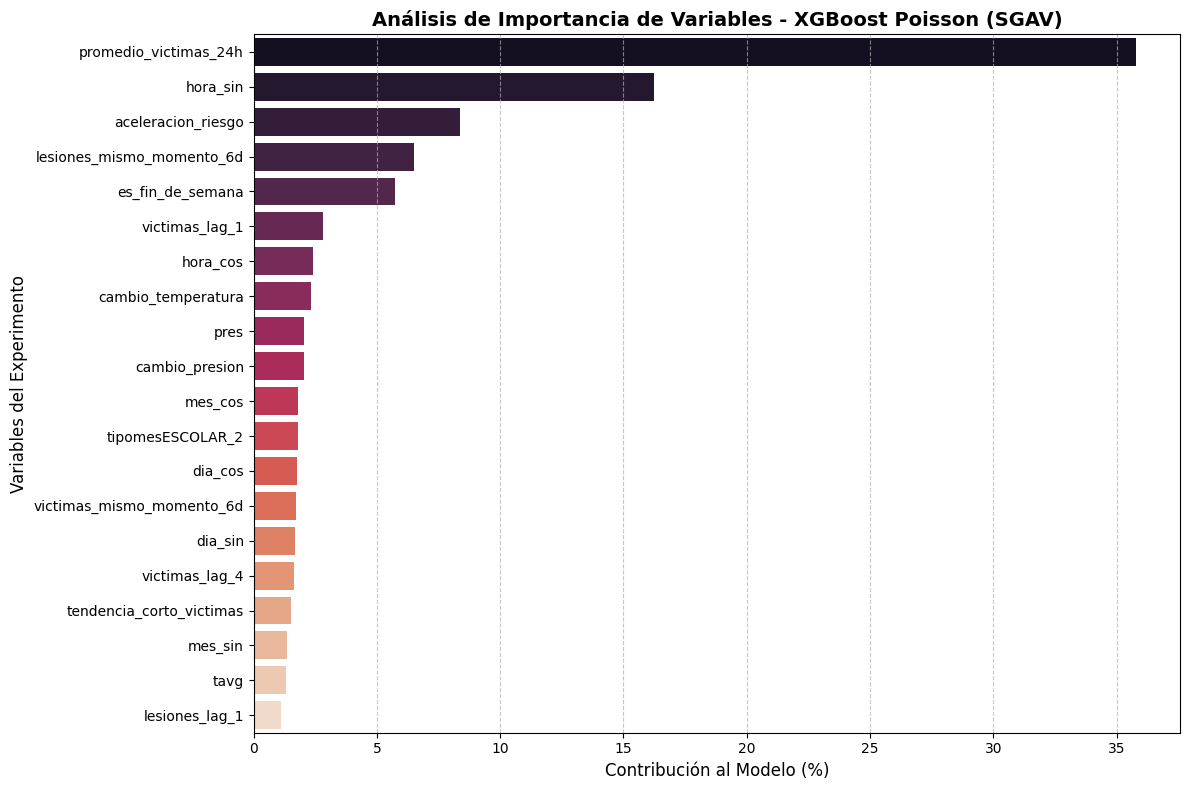
\includegraphics[width=\linewidth]{imagenes/image12.png}
\caption{Contribución de cada variable a la capacidad de predicción del modelo}
\label{fig:contribucion-de-cada-variable-a-la-capac}
\notaflot{\fuentepropia{}, según la salida del modelo entrenado.}
\end{figure}

Los resultados indican que la cantidad de víctimas en promedio en las últimas 24 tiene la mayor contribución a la predicción en orden del \qty{35}{\percent} aproximadamente, le sigue la componente función seno del bloque horario con \qty{15}{\percent} lo que deja entrever que el pasado cercano y el bloque horario en el cual se va a realizar la predicción contribuye a poco más del \qty{50}{\percent} a la predicción del modelo. Se podría afirmar entonces que el riesgo de que existan accidentes depende mayoritariamente de qué pasó en un pasado cercano en términos de cómo vienen evolucionando las víctimas como lo confirma el hecho de que de las primeras 6 variables concentran el \qty{80}{\percent} de la contribución a la predicción, 4 son variables referidas a que pasó y solo 2 están referidas al presente como lo es el caso de la franja horaria (\var{hora\_sin}) y si es fin de semana o no (\var{es\_fin\_de\_semana}).

También se puede observar que otras variables que se pensaban que podían influir notablemente como las climatológicas (\var{cambio\_temperatura}, pres, \var{cambio\_presion}, tavg) no son tan importantes para el modelo en cuestión en términos de aporte a la capacidad de predicción. Obtener esta información es de especial importancia a la hora de desarrollar el producto final, dado que si una variable resulta irrelevante o de baja utilidad puede optarse por no incluirla y en consecuencia no tener que recolectar, procesar, y entregar ese dato al modelo.

\begin{longtable}[]{@{}
>{\raggedright\arraybackslash}p{(\linewidth - 6\tabcolsep) * \real{0.2500}}
  >{\centering\arraybackslash}p{(\linewidth - 6\tabcolsep) * \real{0.2500}}
  >{\centering\arraybackslash}p{(\linewidth - 6\tabcolsep) * \real{0.2500}}
  >{\raggedright\arraybackslash}p{(\linewidth - 6\tabcolsep) * \real{0.2500}}@{}}
\caption{Métricas del modelo para la clase crítica (1) y métricas globales}
\label{tab:metricas-del-modelo-de-clasificacion-par}\\
\toprule\noalign{}
\textbf{Métrica} & \textbf{Porcentaje} & \textbf{Valor Decimal} & \textbf{Interpretación en el Sistema} \\
\midrule\noalign{}
\endfirsthead
\toprule\noalign{}
\textbf{Métrica} & \textbf{Porcentaje} & \textbf{Valor Decimal} & \textbf{Interpretación en el Sistema} \\
\midrule\noalign{}
\endhead
\bottomrule\noalign{}
\endlastfoot
Accuracy Global (Exactitud) & \qty{73.0}{\percent} & 0,73 & Porcentaje global de predicciones correctas sobre el total de casos. \\
Recall (Sensibilidad) en Crítico & \qty{87.4}{\percent} & 0,87 & Porcentaje de eventos críticos capturados. \\
Precisión en Crítico & \qty{77.8}{\percent} & 0,78 & Porcentaje de alertas emitidas que resultaron ser eventos críticos. \\
F1-Score en Crítico & \qty{82.3}{\percent} & 0,82 & Media armónica entre la Precisión y el Recall para la clase crítica. \\
\end{longtable}

\notaflot{Las métricas evalúan el desempeño focalizado en la detección oportuna de eventos de riesgo.}

En la \cref{tab:matriz-de-confusion-del-modelo-de-clasif} se presentaron los resultados agrupados en la matriz de confusión para los 557 datos de testeo; a partir de ellos se calculan las métricas de la \cref{tab:metricas-del-modelo-de-clasificacion-par}.

La exactitud (Accuracy Global) representa el porcentaje de las predicciones correctas (408) sobre los 557 casos de testeo, \qty{73}{\percent} se puede considerar como un buen resultado, pero no hay que perder de vista que representa ese porcentaje respecto de la distribución de la variable objetivo. Como se está intentando predecir un evento crítico como lo es un accidente vial, para los usuarios del producto interesa evaluar la performance específica para ello.

La sensibilidad (Recall) representa en este caso el porcentaje de eventos críticos reales que capturó el modelo, \qty{87.4}{\percent} también se considera un resultado bueno a priori (346 casos de 396). Para complementar esta métrica, se tiene además la precisión, que representa el porcentaje de alertas emitidas por el sistema que efectivamente resultaron ser accidentes en la realidad. Aquí se tiene un punto de especial relevancia dado que la precisión es percibida directamente por el usuario cuando usa el sistema, es decir, que de sí de 445 alarmas 346 son los accidentes reales ese porcentaje también afectará a cómo éste percibe el riesgo cuando ve una alerta. Si el modelo detectara el \qty{100}{\percent} de los accidentes (máximo Recall) emitiendo constantemente alertas entonces esto disminuye la precisión, provocando que el usuario se fatigue y baje la guardia al estar siempre alertado.

El F1-Score es una métrica ampliamente utilizada para evaluar el desempeño de modelos de clasificación, especialmente cuando existe un desbalance entre las clases o cuando resulta igualmente importante minimizar tanto los falsos positivos como los falsos negativos. Esta métrica corresponde a la media armónica entre la Precisión y la Sensibilidad (Recall), por lo que solo alcanza valores elevados cuando ambas presentan un buen desempeño de manera simultánea. A diferencia de la exactitud (Accuracy), el F1-Score ofrece una evaluación más representativa de la capacidad del modelo para identificar correctamente los casos pertenecientes a la clase de interés. En este caso, el F1-Score para la clase \enquote{Crítico} (al menos 1 accidente) alcanzó un valor de \qty{82.3}{\percent}.

\begin{longtable}[]{@{}
>{\raggedright\arraybackslash}p{(\linewidth - 4\tabcolsep) * \real{0.3333}}
  >{\centering\arraybackslash}p{(\linewidth - 4\tabcolsep) * \real{0.3333}}
  >{\raggedright\arraybackslash}p{(\linewidth - 4\tabcolsep) * \real{0.3333}}@{}}
\caption{Desempeño y errores del modelo en la clase normal (0)}
\label{tab:desempeno-y-errores-del-modelo-en-la-cla}\\
\toprule\noalign{}
\textbf{Métrica / Concepto} & \textbf{Valor} & \textbf{Interpretación en el Sistema} \\
\midrule\noalign{}
\endfirsthead
\toprule\noalign{}
\textbf{Métrica / Concepto} & \textbf{Valor} & \textbf{Interpretación en el Sistema} \\
\midrule\noalign{}
\endhead
\bottomrule\noalign{}
\endlastfoot
Recall (Sensibilidad) en Normal & \qty{39.0}{\percent} & Proporción de momentos seguros reales identificados. \\
Falsas Alertas (Falsos Positivos) & 99 & Situaciones sin incidentes en las que el sistema emitió erróneamente una alerta. \\
Críticos No Detectados (Falsos Negativos) & 50 & Situaciones con víctimas reales en las que el sistema omitió activar la alerta. \\
\end{longtable}

En este punto es donde se puede notar la dificultad fundamental de trabajar con predicciones de eventos como los accidentes viales. Cuando se analiza el desempeño para la clase normal (momentos seguros donde no hay accidentes) se tiene una sensibilidad de \qty{39}{\percent} producto de que se identifican correctamente 62 de 161 momentos seguros. Además se tiene 99 falsos positivos y 50 momentos en los cuales no se emite alerta a pesar de que hay víctimas. Estos resultados sugieren que el sistema no puede discriminar con gran capacidad momentos seguros y momentos riesgosos.

El XGBoost que se acaba de describir no es un modelo que pueda ser llevado a producción tal y como está, esto no quiere decir que no sirva, por el contrario, los modelos de línea de base son fundamentales para el desarrollo de productos basados en inteligencia artificial. Este en particular sirvió para generar una referencia para comparar los demas modelos que se entrenen, analizar cuales son las variables que más contribuyen a la capacidad predictiva, analizar qué métricas se deben observar y cuales no, selección de hiperparámetros, entre otros aspectos fundamentales como por ejemplo la forma en la que se agregan los datos que es fundamental no solo para el modelo propiamente dicho sino también a nivel requerimientos del producto final.

\section{Gestión del proyecto}\label{gestiuxf3n-del-proyecto}

\subsection{Definición de Requisitos}\label{definiciuxf3n-de-requisitos}

Para la definición de requisitos se tratan tanto aspectos generales para la gestión de un proyecto como lo pueden ser los objetivos y las partes interesadas como otros que son más específicos de proyectos de software como por ejemplo las restricciones en los datos, los modelos y su despliegue. En la siguiente sección se mencionan de forma resumida los principales requisitos que se relevaron y como se definieron, al final de la misma se podrá tener una idea de los objetivos, partes interesadas, restricciones de los datos y de los modelos, requisitos funcionales y no funcionales.

El objetivo de este proyecto es obtener un sistema que basado en el uso de inteligencia artificial permite tomar mejores decisiones a usuarios específicos del Ministerio Público Fiscal, en concreto los que trabajan en el área de accidentología vial. En este sentido también es válido aclarar para quien no es este producto, no es para personal de policía judicial, agentes de tránsito, personal municipal, ni ciudadanos en general. Teniendo esto en cuenta también se pueden definir las partes interesadas, a saber: Ministerio Público Fiscal, MPF Accidentología Vial, MPF Formación, LIDeSIA y FCEFyN.

Para poder alcanzar adecuadamente estos objetivos primero se deben establecer una serie de supuestos respecto de las restricciones que imponen los modelos para series temporales. Un algoritmo que predice el riesgo de accidentes viales generalmente necesita información en bloques discretos de tiempo, como por ejemplo en el caso de LightGBM y XGB, es decir que se requiere que los usuarios finales mantengan permanentemente actualizados los datos que son inputs para el modelo. En este proyecto, los bloques de predicción son de 6 horas y por lo tanto necesitamos poder agregar todos los datos conocidos en ese intervalo para poder realizar la predicción. Existen otros modelos que son más flexibles con este requerimiento, pero aquí hay que tener en cuenta otra restricción fundamental. Siendo que se está desarrollando el producto de forma tal que esté alineado con las normas ISO 42001 es necesario seleccionar un modelo que sea explicable (XAI). Se tiene entonces que asumir esta restricción y dar por supuesto que el equipo del MPF se compromete a mantener los datos actualizados.

En este punto es importante destacar que el alcance que se definió para la gestión de este proyecto es el acorde a un producto mínimo viable, es decir que si bien no se incluyen todas las características funcionales y no funcionales en el desarrollo (control de acceso basado en roles, cumplimiento de todos los puntos de las normas ISO 42001, Ciberseguridad, UX UI, etc), se trabaja teniendo en cuenta que en el futuro serán obligatorias y que por lo tanto se debe diseñar sin generar incompatibilidades.

En cuanto a la necesidad de realizar \eng{forecasting}, se justifica bajo la referencia B.6.2.2a (Requisitos y especificaciones del sistema de IA), surge como una evolución deseable del actual sistema de gestión descriptivo para pasar de la caracterización a la predicción. Estas especificaciones funcionales se traducen en un sistema de alerta temprana basado en la escala del puntaje estándar Z-score, el cual activa una alerta roja si el riesgo predicho supera las dos desviaciones estándar respecto al promedio, una alerta naranja si se ubica entre una y media y dos desviaciones, una alerta amarilla entre una y una y media desviaciones, y una alerta verde si la situación está controlada con un riesgo menor o igual a una desviación estándar.

\subsection{Dependencias tecnológicas y funcionales}\label{dependencias-tecnoluxf3gicas-y-funcionales}

Las dependencias tecnológicas y funcionales aplicables a un proyecto de software basado en inteligencia artificial pueden ser sumamente extensas dependiendo de la complejidad del sistema, dado que en este caso estamos analizando un MVP se tendrán en cuenta sólo las aplicables al alcance de una prueba de concepto de estas características.

Primeramente se deben analizar las dependencias funcionales, es decir, todas las condiciones del negocio o los procesos operativos en los cuales la intervención humana es necesaria para que el producto o sistema funcione. Se tiene por ejemplo el caso de la carga de datos, una falla en este proceso es vital para el sistema, si la información no se carga a tiempo o se introducen datos erróneos el resultado puede ser de impacto crítico en el caso de lo primero (el sistema queda inutilizable) o de impacto medio en el segundo caso (el sistema funciona pero con precisión reducida).

Por otra parte se tienen las dependencias tecnológicas, que son los componentes de hardware, software, servicios en la nube, APIs o bases de datos de los que depende la solución para recopilar datos, entrenar modelos o mostrar resultados. Con el mismo criterio mencionado anteriormente se destaca el Centro de Cómputos de Alto Desempeño, tanto en su servidor donde se aloja el servicio web como sus clusters de cómputo como Serafin o Mendieta donde se entrenan los modelos. El servidor de CCAD donde se aloja el servicio genera una dependencia crítica porque sin él es imposible alertar a los usuarios del MPF, en cambio, los clusters donde se entrenan los modelos no generan un impacto que comprometa al sistema dado que no es necesario reentrenar constantemente para mantener la precisión. Por último se encuentra una dependencia referida al consumo de APIs meteorológicas para la extracción de datos climáticos necesarios para realizar las predicciones, si bien es posible configurar el sistema para que tenga APIs como segunda opción (si la principal se cae), el impacto es bajo ya que no tener esta información disponible no reduce de manera significativa el desempeño del modelo.

\begin{longtable}[]{@{}
>{\raggedright\arraybackslash}p{(\linewidth - 4\tabcolsep) * \real{0.2281}}
  >{\raggedright\arraybackslash}p{(\linewidth - 4\tabcolsep) * \real{0.1927}}
  >{\raggedright\arraybackslash}p{(\linewidth - 4\tabcolsep) * \real{0.5428}}@{}}
\caption{Matriz de dependencias}
\label{tab:matriz-de-dependencias}\\
\toprule\noalign{}
\textbf{Dependencia} & \textbf{Tipo} & \textbf{Impacto} \\
\midrule\noalign{}
\endfirsthead
\toprule\noalign{}
\textbf{Dependencia} & \textbf{Tipo} & \textbf{Impacto} \\
\midrule\noalign{}
\endhead
\bottomrule\noalign{}
\endlastfoot
Carga de Datos & Funcional & Crítica: Se pierde la secuencialidad del modelo \\
Clasificacion Lesión & Funcional & Media: El modelo pierde precisión \\
CCAD Servidor & Tecnológica & Critica: El modelo no está disponible \\
CCAD Serafin & Tecnológica & Baja: Impide el reentrenamiento del modelo \\
API Meteo & Tecnológica & Media: El modelo pierde precisión \\
\end{longtable}

\notaflot{\fuentepropia{}.}

\subsection{Gestión de riesgos}\label{gestiuxf3n-de-riesgos}

La gestión de riesgos del sistema de Alerta Temprana de Accidentes Viales se estructuró siguiendo los lineamientos de la cláusula 6,1 de la norma ISO/IEC 42001:2023 a nivel general y por otro lado a la orientación metodológica de la norma ISO/IEC 23894:2023. La primera establece qué debe producir el proceso en términos de criterios definidos, una evaluación con resultados comparables, un plan de tratamiento y una evaluación de impacto. Mientras que la segunda aporta el procedimiento y, en particular, el relevamiento de fuentes de riesgo de su Anexo B, empleado en este documento como marco de identificación.

Es necesario distinguir dos ejercicios que la norma 42001 requiere por separado y que con frecuencia se confunden. La cláusula 6.1.2 refiere a la evaluación de los riesgos que afectan a los objetivos de la organización, mientras que la cláusula 6.1.4 refiere a la evaluación del impacto del sistema sobre individuos, grupos y sociedad. El presente apartado desarrolla el primero; el segundo se trata en el apartado siguiente. La relación entre ambos es de alimentación: los impactos identificados sobre terceros se incorporan al registro de riesgos en la medida en que generan exposición institucional, legal o reputacional para los organismos involucrados.

El alcance de esta evaluación comprende el ciclo completo del dato y de la predicción bajo el esquema de trabajo que se definió previamente a lo largo de este documento, que es de responsabilidad compartida: el Ministerio Público Fiscal es el origen de los datos y el destinatario de las alertas, mientras que el Laboratorio de Investigación y Desarrollo de Software e Inteligencia Artificial concentra el procesamiento, el entrenamiento y la generación de las predicciones. Al no delegar completamente la operación del sistema en su conjunto, se generan dos superficies de riesgo propias y se tratan como tales, el ingreso de datos y la emisión de alertas.

\subsection{Criterios de Riesgo}\label{criterios-de-riesgo}

Con el fin de que la evaluación produzca resultados comparables entre sí, se definieron escalas cualitativas de cuatro niveles para la probabilidad de ocurrencia y para la severidad del impacto. Se optó por cuatro niveles en lugar de los tres habituales para mantener coherencia con la codificación de cuatro colores adoptada por la capa de decisión del propio sistema. El nivel de riesgo resultante se obtiene del producto de ambos valores.

\begin{longtable}[]{@{}
>{\raggedright\arraybackslash}p{(\linewidth - 4\tabcolsep) * \real{0.1606}}
  >{\centering\arraybackslash}p{(\linewidth - 4\tabcolsep) * \real{0.0964}}
  >{\raggedright\arraybackslash}p{(\linewidth - 4\tabcolsep) * \real{0.7066}}@{}}
\caption{Escala de probabilidad de ocurrencia}
\label{tab:escala-de-probabilidad-de-ocurrencia}\\
\toprule\noalign{}
\textbf{Nivel} & \textbf{Valor} & \textbf{Criterio de asignación} \\
\midrule\noalign{}
\endfirsthead
\toprule\noalign{}
\textbf{Nivel} & \textbf{Valor} & \textbf{Criterio de asignación} \\
\midrule\noalign{}
\endhead
\bottomrule\noalign{}
\endlastfoot
Baja & 1 & No se ha observado durante el desarrollo y no existen indicios de que pueda materializarse en el horizonte del prototipo. \\
Media & 2 & Es plausible; existen condiciones que podrían habilitarla, aunque no se ha manifestado. \\
Alta & 3 & Se ha manifestado de forma ocasional durante el desarrollo o es esperable en condiciones normales de operación. \\
Muy alta & 4 & Se verifica de manera sistemática en la situación actual del proyecto. \\
\end{longtable}

\notaflot{\fuentepropia{} sobre la base de ISO/IEC 23894:2023.}

\begin{longtable}[]{@{}
>{\raggedright\arraybackslash}p{(\linewidth - 4\tabcolsep) * \real{0.1606}}
  >{\centering\arraybackslash}p{(\linewidth - 4\tabcolsep) * \real{0.0964}}
  >{\raggedright\arraybackslash}p{(\linewidth - 4\tabcolsep) * \real{0.7066}}@{}}
\caption{Escala de severidad del impacto}
\label{tab:escala-de-severidad-del-impacto}\\
\toprule\noalign{}
\textbf{Nivel} & \textbf{Valor} & \textbf{Criterio de asignación} \\
\midrule\noalign{}
\endfirsthead
\toprule\noalign{}
\textbf{Nivel} & \textbf{Valor} & \textbf{Criterio de asignación} \\
\midrule\noalign{}
\endhead
\bottomrule\noalign{}
\endlastfoot
Menor & 1 & Afecta la comodidad del desarrollo sin comprometer resultados ni usuarios. \\
Moderado & 2 & Degrada el desempeño del sistema o retrasa el cronograma, sin invalidar los resultados obtenidos. \\
Mayor & 3 & Invalida resultados, inutiliza temporalmente el sistema o afecta la confianza del usuario final en la herramienta. \\
Crítico & 4 & Compromete derechos de terceros, obligaciones legales del organismo o la viabilidad del proyecto. \\
\end{longtable}

\notaflot{\fuentepropia{} sobre la base de ISO/IEC 23894:2023.}

\begin{longtable}[]{@{}
>{\raggedright\arraybackslash}p{(\linewidth - 8\tabcolsep) * \real{0.1931}}
  >{\centering\arraybackslash}p{(\linewidth - 8\tabcolsep) * \real{0.1931}}
  >{\centering\arraybackslash}p{(\linewidth - 8\tabcolsep) * \real{0.1931}}
  >{\centering\arraybackslash}p{(\linewidth - 8\tabcolsep) * \real{0.1931}}
  >{\centering\arraybackslash}p{(\linewidth - 8\tabcolsep) * \real{0.1931}}@{}}
\caption{Matriz de nivel de riesgo}
\label{tab:matriz-de-nivel-de-riesgo}\\
\toprule\noalign{}
\textbf{Probabilidad / Impacto} & \textbf{Menor (1)} & \textbf{Moderado (2)} & \textbf{Mayor (3)} & \textbf{Crítico (4)} \\
\midrule\noalign{}
\endfirsthead
\toprule\noalign{}
\textbf{Probabilidad / Impacto} & \textbf{Menor (1)} & \textbf{Moderado (2)} & \textbf{Mayor (3)} & \textbf{Crítico (4)} \\
\midrule\noalign{}
\endhead
\bottomrule\noalign{}
\endlastfoot
Muy alta (4) & Amarillo (4) & Naranja (8) & Rojo (12) & Rojo (16) \\
Alta (3) & Verde (3) & Amarillo (6) & Naranja (9) & Rojo (12) \\
Media (2) & Verde (2) & Amarillo (4) & Amarillo (6) & Naranja (8) \\
Baja (1) & Verde (1) & Verde (2) & Verde (3) & Amarillo (4) \\
\end{longtable}

\notaflot{\fuentepropia{}. El valor entre paréntesis corresponde al producto de la probabilidad por el impacto.}

Respecto del nivel de riesgo declarado para la etapa actual se define en función del nivel de madurez tecnológica. Al tratarse de un prototipo en TRL 3 que no se encuentra desplegado en operación real y que no sustituye ningún procedimiento vigente del organismo, se aceptan sin acción los riesgos de nivel verde y amarillo. Los riesgos de nivel naranja se documentan con un tratamiento previsto que puede posponerse a etapas de mayor madurez. Los riesgos de nivel rojo requieren tratamiento explícito o, en su defecto, una declaración de aceptación fundamentada, y constituyen condición de salida hacia niveles TRL superiores.

\subsection{Identificación y Valoración de Riesgos}\label{identificaciuxf3n-y-valoraciuxf3n-de-riesgos}

La identificación se realizó recorriendo el catálogo de fuentes de riesgo del Anexo B de la norma ISO/IEC 23894:2023 y contrastando cada categoría contra las características concretas del sistema desarrollado. El relevamiento incorpora además las dependencias funcionales y tecnológicas documentadas en el apartado anterior, que constituyen la base de los riesgos R8 y R9. El resultado se presenta en la \cref{tab:registro-de-identificacion-y-valoracion-}.

\begin{longtable}[]{@{}
>{\raggedright\arraybackslash}p{(\linewidth - 10\tabcolsep) * \real{0.0698}}
  >{\raggedright\arraybackslash}p{(\linewidth - 10\tabcolsep) * \real{0.3813}}
  >{\raggedright\arraybackslash}p{(\linewidth - 10\tabcolsep) * \real{0.2524}}
  >{\centering\arraybackslash}p{(\linewidth - 10\tabcolsep) * \real{0.0483}}
  >{\centering\arraybackslash}p{(\linewidth - 10\tabcolsep) * \real{0.0483}}
  >{\centering\arraybackslash}p{(\linewidth - 10\tabcolsep) * \real{0.1665}}@{}}
\caption{Registro de identificación y valoración de riesgos}
\label{tab:registro-de-identificacion-y-valoracion-}\\
\toprule\noalign{}
\textbf{ID} & \textbf{Descripción del riesgo} & \textbf{Fuente de riesgo (Anexo B, ISO/IEC 23894)} & \textbf{P} & \textbf{I} & \textbf{Nivel} \\
\midrule\noalign{}
\endfirsthead
\toprule\noalign{}
\textbf{ID} & \textbf{Descripción del riesgo} & \textbf{Fuente de riesgo (Anexo B, ISO/IEC 23894)} & \textbf{P} & \textbf{I} & \textbf{Nivel} \\
\midrule\noalign{}
\endhead
\bottomrule\noalign{}
\endlastfoot
R1 & Errores de transcripción y falta de normalización derivados de la carga manual de los siniestros por parte del personal administrativo. & Calidad y procedencia de los datos & 3 & 3 & Naranja (9) \\
R2 & Latencia entre la ocurrencia del siniestro y su digitalización, que altera la posición temporal del evento en la serie. & Calidad de los datos / Complejidad del entorno & 4 & 3 & Rojo (12) \\
R3 & Sesgo de subregistro: la base contiene únicamente siniestros con intervención judicial y no representa la siniestralidad total de la ciudad. & Sesgo algorítmico & 4 & 2 & Naranja (8) \\
R4 & Reidentificación de personas involucradas por cruce de fecha, franja horaria, georreferenciación y tipo de lesión, no verificada hasta la fecha. & Privacidad y protección de datos & 3 & 4 & Rojo (12) \\
R5 & Fatiga de alerta por exceso de falsos positivos, con la consiguiente pérdida de confianza del usuario en la herramienta. & Nivel de automatización / Uso del sistema & 3 & 3 & Naranja (9) \\
R6 & Sesgo de automatización: delegación del juicio profesional en la salida del sistema sin contraste con otras fuentes. & Nivel de automatización & 2 & 3 & Amarillo (6) \\
R7 & Ausencia de un procedimiento formalizado de supervisión humana para validar o desestimar las alertas antes de su uso. & Supervisión humana / Uso del sistema & 3 & 3 & Naranja (9) \\
R8 & Indisponibilidad del servidor del CCAD que aloja el servicio, con interrupción total de la emisión de alertas. & Hardware e infraestructura & 2 & 3 & Amarillo (6) \\
R9 & Interrupción del suministro de datos climáticos por caída de la API meteorológica. & Complejidad del entorno de despliegue & 2 & 2 & Amarillo (4) \\
R10 & Uso desviado del sistema hacia finalidades no previstas, riesgo latente que se activaría con la incorporación de predicción georreferenciada por zonas. & Uso previsto / Impacto social & 2 & 3 & Amarillo (6) \\
R11 & Dependencia de personas clave y ausencia de un esquema definido de continuidad o transferencia del sistema. & Ciclo de vida del sistema de IA & 3 & 2 & Amarillo (6) \\
\end{longtable}

\notaflot{\fuentepropia{}. P: probabilidad; I: impacto, valorados según las \cref{tab:escala-de-probabilidad-de-ocurrencia,tab:escala-de-severidad-del-impacto}. El nivel resulta de la \cref{tab:matriz-de-nivel-de-riesgo}. Las categorías de fuente corresponden al Anexo B de ISO/IEC 23894:2023. Los riesgos R8 y R9 se corresponden con las dependencias de impacto crítico y medio identificadas en la matriz de dependencias tecnológicas y funcionales.}

\subsection{Plan de Mitigación de Riesgos}\label{plan-de-mitigacion-de-riesgos}

La \cref{tab:plan-de-mitigacion-de-riesgos} consigna el tratamiento propuesto para cada riesgo identificado y el nivel residual estimado al cierre de la etapa actual. Se indica asimismo el actor responsable, considerando el esquema de responsabilidad compartida mencionado al inicio del apartado.

\begin{longtable}[]{@{}
>{\raggedright\arraybackslash}p{(\linewidth - 6\tabcolsep) * \real{0.0697}}
  >{\raggedright\arraybackslash}p{(\linewidth - 6\tabcolsep) * \real{0.4770}}
  >{\raggedright\arraybackslash}p{(\linewidth - 6\tabcolsep) * \real{0.1768}}
  >{\raggedright\arraybackslash}p{(\linewidth - 6\tabcolsep) * \real{0.2412}}@{}}
\caption{Plan de mitigación de riesgos}
\label{tab:plan-de-mitigacion-de-riesgos}\\
\toprule\noalign{}
\textbf{ID} & \textbf{Tratamiento propuesto} & \textbf{Responsable} & \textbf{Residual en TRL 3} \\
\midrule\noalign{}
\endfirsthead
\toprule\noalign{}
\textbf{ID} & \textbf{Tratamiento propuesto} & \textbf{Responsable} & \textbf{Residual en TRL 3} \\
\midrule\noalign{}
\endhead
\bottomrule\noalign{}
\endlastfoot
R1 & Reducir. Validaciones automáticas de rango y consistencia en la etapa de curado, y documentación del diccionario de datos acordada con el equipo de datos del MPF. & LIDeSIA / Equipo de datos del MPF & Amarillo. Aceptado. \\
R2 & Reducir. Incorporación de la fecha de digitalización como variable de control, evaluación del desfase medio y definición de una ventana de corte que excluya los bloques aún incompletos. & LIDeSIA / MPF & Naranja. Condición de salida hacia TRL 4. \\
R3 & Aceptar con declaración. La población objetivo del sistema son precisamente los eventos con intervención judicial, por lo que el sesgo resulta parcialmente alineado con el caso de uso. Se documenta como limitación de generalización. & LIDeSIA & Naranja. Aceptado con declaración. \\
R4 & Reducir. Verificación de unicidad de los registros por combinación de cuasi-identificadores y, en caso de detectarse casos únicos, agregación espacial o temporal previa a cualquier publicación o difusión del conjunto de datos. & LIDeSIA / MPF & Rojo. Tratamiento pendiente y condición de salida hacia TRL 4. \\
R5 & Reducir. Calibración del umbral de decisión priorizando la precisión por sobre la sensibilidad, con aceptación explícita de la consecuencia que ello implica sobre los eventos no detectados, conforme a la política declarada en el apartado siguiente. & LIDeSIA & Amarillo. Tratamiento en curso. \\
R6 & Reducir. Comunicación de la alerta acompañada de su intervalo de predicción y no como valor puntual, y declaración del carácter complementario del sistema respecto del procedimiento vigente, de modo que la incertidumbre resulte visible para el usuario. & LIDeSIA & Amarillo. Aceptado. \\
R7 & Reducir, de forma compartida y diferida. Definición de un procedimiento de validación humana previa a la actuación, con registro de la decisión adoptada, prevista para la etapa de integración con el MPF. & MPF / LIDeSIA & Naranja. Condición de salida hacia TRL 4. \\
R8 & Aceptar con tratamiento diferido. Definición del requisito de disponibilidad y del esquema de contingencia prevista para la etapa de despliegue. & CCAD / LIDeSIA & Amarillo. Aceptado. \\
R9 & Evitar. Dado que el análisis de importancia de variables del modelo de línea de base evidenció una contribución marginal de las variables climáticas, se evalúa su exclusión del conjunto de entradas, lo que elimina la fuente de riesgo. Como alternativa, configuración de una fuente meteorológica secundaria. & LIDeSIA & Verde, sujeto a la confirmación de la exclusión de la variable. \\
R10 & Evitar. Declaración explícita del uso previsto y de los usos no admitidos del sistema, incorporada al apartado de definición de requisitos, y nueva evaluación de impacto como condición previa a la incorporación de predicción georreferenciada. & LIDeSIA / MPF & Amarillo. Latente. \\
R11 & Reducir. Documentación del código y de los procedimientos en repositorio versionado, como condición previa a cualquier esquema de transferencia. & LIDeSIA & Amarillo. Aceptado. \\
\end{longtable}

\notaflot{\fuentepropia{}. Las opciones de tratamiento corresponden a las categorías de ISO 31000:2018 adoptadas por ISO/IEC 23894:2023: evitar la fuente de riesgo, reducir la probabilidad o la consecuencia, compartir el riesgo con un tercero y aceptar el riesgo de forma informada. El nivel residual se estima al cierre de la etapa actual de madurez tecnológica.}

\subsection{Evaluación del Impacto del Sistema de IA}\label{evaluaciuxf3n-del-impacto-del-sistema-de-ia}

La cláusula 6.1.4 de la norma ISO/IEC 42001:2023, desarrollada en los apartados A.5 y B.5 de sus anexos, requiere evaluar las consecuencias del sistema sobre individuos, grupos y sociedad, con independencia del riesgo que el sistema representa para los objetivos de la organización. La norma ISO/IEC 42005:2024 provee orientación específica sobre este tema en cuestión. La evaluación que sigue corresponde al estado actual del prototipo y debe repetirse en caso de haber cambios en el sistema o en su contexto de uso.

\subsection{Impacto Sobre Individuos y Grupos}\label{impacto-sobre-individuos-y-grupos}

El sistema no elabora perfiles individuales ni produce decisiones que afecten a personas en específico, es decir, la unidad de predicción es un bloque temporal de seis horas para el conjunto de toda la ciudad, y la salida es una estimación agregada de siniestralidad. En consecuencia, no se identifican decisiones automatizadas de efecto individual en el sentido de la normativa de protección de datos.

El impacto sobre individuos se concentra, por lo tanto, en el tratamiento de los datos de origen. La base fue anonimizada mediante la supresión de los nombres de las personas involucradas, conforme a lo previsto por la Ley N.º 25.326 de Protección de los Datos Personales. No obstante, la anonimización de identificadores directos no elimina por sí sola la posibilidad de reidentificación por cruce de cuasi-identificadores, y esta verificación no se realizó durante el desarrollo del prototipo. Se trata de una limitación reconocida, registrada como riesgo R4 y con tratamiento pendiente, que constituye condición previa a cualquier difusión del conjunto de datos fuera del ámbito de LIDeSIA.

Respecto al impacto sobre grupos, en su configuración actual el sistema opera sobre la totalidad de la ciudad de Córdoba sin segregación territorial, por lo que no produce salidas susceptibles de asociarse a un barrio, una zona o una población determinada.

\subsection{Conclusión de la Evaluación}\label{conclusiuxf3n-de-la-evaluaciuxf3n}

El nivel de riesgo residual del prototipo resulta aceptable para el nivel de madurez tecnológica TRL 3, en tanto el sistema todavía no se encuentra desplegado, no sustituye ningún procedimiento del organismo y sus salidas no alcanzan a individuos ni a grupos determinados. Esta aceptación no se extiende a niveles superiores, los riesgos R2, R4 y R11 se establecen como condiciones de salida, es decir, deben encontrarse tratados con anterioridad a cualquier prueba en entorno operativo real.

\subsection{Flujograma de procesos}\label{flujograma-de-procesos}

\begin{figure}[htbp]
\centering

\includegraphics[width=\linewidth]{imagenes/image66.png}
\caption{Flujograma del proceso}
\label{fig:flujograma-del-proceso}
\notaflot{\fuentepropia{}.}
\end{figure}
